% Options for packages loaded elsewhere
\PassOptionsToPackage{unicode}{hyperref}
\PassOptionsToPackage{hyphens}{url}
%
\documentclass[
]{article}
\title{\texttt{pybats-detection}: A python package for outlier and
structural changes detection in time series analysis}
\author{André Menezes and Eduardo Gabriel}
\date{31 março, 2022}

\usepackage{amsmath,amssymb}
\usepackage{lmodern}
\usepackage{iftex}
\ifPDFTeX
  \usepackage[T1]{fontenc}
  \usepackage[utf8]{inputenc}
  \usepackage{textcomp} % provide euro and other symbols
\else % if luatex or xetex
  \usepackage{unicode-math}
  \defaultfontfeatures{Scale=MatchLowercase}
  \defaultfontfeatures[\rmfamily]{Ligatures=TeX,Scale=1}
\fi
% Use upquote if available, for straight quotes in verbatim environments
\IfFileExists{upquote.sty}{\usepackage{upquote}}{}
\IfFileExists{microtype.sty}{% use microtype if available
  \usepackage[]{microtype}
  \UseMicrotypeSet[protrusion]{basicmath} % disable protrusion for tt fonts
}{}
\makeatletter
\@ifundefined{KOMAClassName}{% if non-KOMA class
  \IfFileExists{parskip.sty}{%
    \usepackage{parskip}
  }{% else
    \setlength{\parindent}{0pt}
    \setlength{\parskip}{6pt plus 2pt minus 1pt}}
}{% if KOMA class
  \KOMAoptions{parskip=half}}
\makeatother
\usepackage{xcolor}
\IfFileExists{xurl.sty}{\usepackage{xurl}}{} % add URL line breaks if available
\IfFileExists{bookmark.sty}{\usepackage{bookmark}}{\usepackage{hyperref}}
\hypersetup{
  pdftitle={pybats-detection: A python package for outlier and structural changes detection in time series analysis},
  pdfauthor={André Menezes and Eduardo Gabriel},
  hidelinks,
  pdfcreator={LaTeX via pandoc}}
\urlstyle{same} % disable monospaced font for URLs
\usepackage[margin=1in]{geometry}
\usepackage{color}
\usepackage{fancyvrb}
\newcommand{\VerbBar}{|}
\newcommand{\VERB}{\Verb[commandchars=\\\{\}]}
\DefineVerbatimEnvironment{Highlighting}{Verbatim}{commandchars=\\\{\}}
% Add ',fontsize=\small' for more characters per line
\usepackage{framed}
\definecolor{shadecolor}{RGB}{248,248,248}
\newenvironment{Shaded}{\begin{snugshade}}{\end{snugshade}}
\newcommand{\AlertTok}[1]{\textcolor[rgb]{0.94,0.16,0.16}{#1}}
\newcommand{\AnnotationTok}[1]{\textcolor[rgb]{0.56,0.35,0.01}{\textbf{\textit{#1}}}}
\newcommand{\AttributeTok}[1]{\textcolor[rgb]{0.77,0.63,0.00}{#1}}
\newcommand{\BaseNTok}[1]{\textcolor[rgb]{0.00,0.00,0.81}{#1}}
\newcommand{\BuiltInTok}[1]{#1}
\newcommand{\CharTok}[1]{\textcolor[rgb]{0.31,0.60,0.02}{#1}}
\newcommand{\CommentTok}[1]{\textcolor[rgb]{0.56,0.35,0.01}{\textit{#1}}}
\newcommand{\CommentVarTok}[1]{\textcolor[rgb]{0.56,0.35,0.01}{\textbf{\textit{#1}}}}
\newcommand{\ConstantTok}[1]{\textcolor[rgb]{0.00,0.00,0.00}{#1}}
\newcommand{\ControlFlowTok}[1]{\textcolor[rgb]{0.13,0.29,0.53}{\textbf{#1}}}
\newcommand{\DataTypeTok}[1]{\textcolor[rgb]{0.13,0.29,0.53}{#1}}
\newcommand{\DecValTok}[1]{\textcolor[rgb]{0.00,0.00,0.81}{#1}}
\newcommand{\DocumentationTok}[1]{\textcolor[rgb]{0.56,0.35,0.01}{\textbf{\textit{#1}}}}
\newcommand{\ErrorTok}[1]{\textcolor[rgb]{0.64,0.00,0.00}{\textbf{#1}}}
\newcommand{\ExtensionTok}[1]{#1}
\newcommand{\FloatTok}[1]{\textcolor[rgb]{0.00,0.00,0.81}{#1}}
\newcommand{\FunctionTok}[1]{\textcolor[rgb]{0.00,0.00,0.00}{#1}}
\newcommand{\ImportTok}[1]{#1}
\newcommand{\InformationTok}[1]{\textcolor[rgb]{0.56,0.35,0.01}{\textbf{\textit{#1}}}}
\newcommand{\KeywordTok}[1]{\textcolor[rgb]{0.13,0.29,0.53}{\textbf{#1}}}
\newcommand{\NormalTok}[1]{#1}
\newcommand{\OperatorTok}[1]{\textcolor[rgb]{0.81,0.36,0.00}{\textbf{#1}}}
\newcommand{\OtherTok}[1]{\textcolor[rgb]{0.56,0.35,0.01}{#1}}
\newcommand{\PreprocessorTok}[1]{\textcolor[rgb]{0.56,0.35,0.01}{\textit{#1}}}
\newcommand{\RegionMarkerTok}[1]{#1}
\newcommand{\SpecialCharTok}[1]{\textcolor[rgb]{0.00,0.00,0.00}{#1}}
\newcommand{\SpecialStringTok}[1]{\textcolor[rgb]{0.31,0.60,0.02}{#1}}
\newcommand{\StringTok}[1]{\textcolor[rgb]{0.31,0.60,0.02}{#1}}
\newcommand{\VariableTok}[1]{\textcolor[rgb]{0.00,0.00,0.00}{#1}}
\newcommand{\VerbatimStringTok}[1]{\textcolor[rgb]{0.31,0.60,0.02}{#1}}
\newcommand{\WarningTok}[1]{\textcolor[rgb]{0.56,0.35,0.01}{\textbf{\textit{#1}}}}
\usepackage{longtable,booktabs,array}
\usepackage{calc} % for calculating minipage widths
% Correct order of tables after \paragraph or \subparagraph
\usepackage{etoolbox}
\makeatletter
\patchcmd\longtable{\par}{\if@noskipsec\mbox{}\fi\par}{}{}
\makeatother
% Allow footnotes in longtable head/foot
\IfFileExists{footnotehyper.sty}{\usepackage{footnotehyper}}{\usepackage{footnote}}
\makesavenoteenv{longtable}
\usepackage{graphicx}
\makeatletter
\def\maxwidth{\ifdim\Gin@nat@width>\linewidth\linewidth\else\Gin@nat@width\fi}
\def\maxheight{\ifdim\Gin@nat@height>\textheight\textheight\else\Gin@nat@height\fi}
\makeatother
% Scale images if necessary, so that they will not overflow the page
% margins by default, and it is still possible to overwrite the defaults
% using explicit options in \includegraphics[width, height, ...]{}
\setkeys{Gin}{width=\maxwidth,height=\maxheight,keepaspectratio}
% Set default figure placement to htbp
\makeatletter
\def\fps@figure{htbp}
\makeatother
\setlength{\emergencystretch}{3em} % prevent overfull lines
\providecommand{\tightlist}{%
  \setlength{\itemsep}{0pt}\setlength{\parskip}{0pt}}
\setcounter{secnumdepth}{-\maxdimen} % remove section numbering
\ifLuaTeX
  \usepackage{selnolig}  % disable illegal ligatures
\fi

\begin{document}
\maketitle

\hypertarget{smoothing}{%
\section{Smoothing}\label{smoothing}}

To demonstrate the use of the Smoothing class we will start with a
simulated example in which a sequence of observations
\(y_1, \dots, y_t\) were generated following DLM evolution structure
given by

\[
y_t &=& \textbf{F} \boldsymbol{\theta}_t + \epsilon_t, \quad \epsilon_t \sim N[0, V_t], \\
\boldsymbol{\theta}_t &=& \mathbf{G} \boldsymbol{\theta}_{t-1} + \omega_t, \quad \omega_t \sim N[0, W_t]
\]

This can be done using the \texttt{RandomDLM} class which has the
arguments (n, V, W): the number of observations, observational variance
and state vector variance. This class has three methods that simulate
data using different mechanisms:

For now, we stick with \texttt{.level}, simulating \(n=100\)
observations with both observational and state vector variance equals to
one \(1\), the starting level is set to \(100\). The simulated data is
plotted below.

\begin{Shaded}
\begin{Highlighting}[]
\OperatorTok{\textgreater{}\textgreater{}\textgreater{}} \CommentTok{\# Generating level data model}
\OperatorTok{\textgreater{}\textgreater{}\textgreater{}}\NormalTok{ np.random.seed(}\DecValTok{66}\NormalTok{)}
\OperatorTok{\textgreater{}\textgreater{}\textgreater{}}\NormalTok{ rdlm }\OperatorTok{=}\NormalTok{ RandomDLM(n}\OperatorTok{=}\DecValTok{100}\NormalTok{, V}\OperatorTok{=}\DecValTok{1}\NormalTok{, W}\OperatorTok{=}\DecValTok{1}\NormalTok{)}
\OperatorTok{\textgreater{}\textgreater{}\textgreater{}}\NormalTok{ df\_simulated }\OperatorTok{=}\NormalTok{ rdlm.level(start\_level}\OperatorTok{=}\DecValTok{100}\NormalTok{, dict\_shift}\OperatorTok{=}\NormalTok{\{\})}
\OperatorTok{\textgreater{}\textgreater{}\textgreater{}}\NormalTok{ y }\OperatorTok{=}\NormalTok{ df\_simulated[}\StringTok{"y"}\NormalTok{]}
\end{Highlighting}
\end{Shaded}

\begin{figure}

{\centering 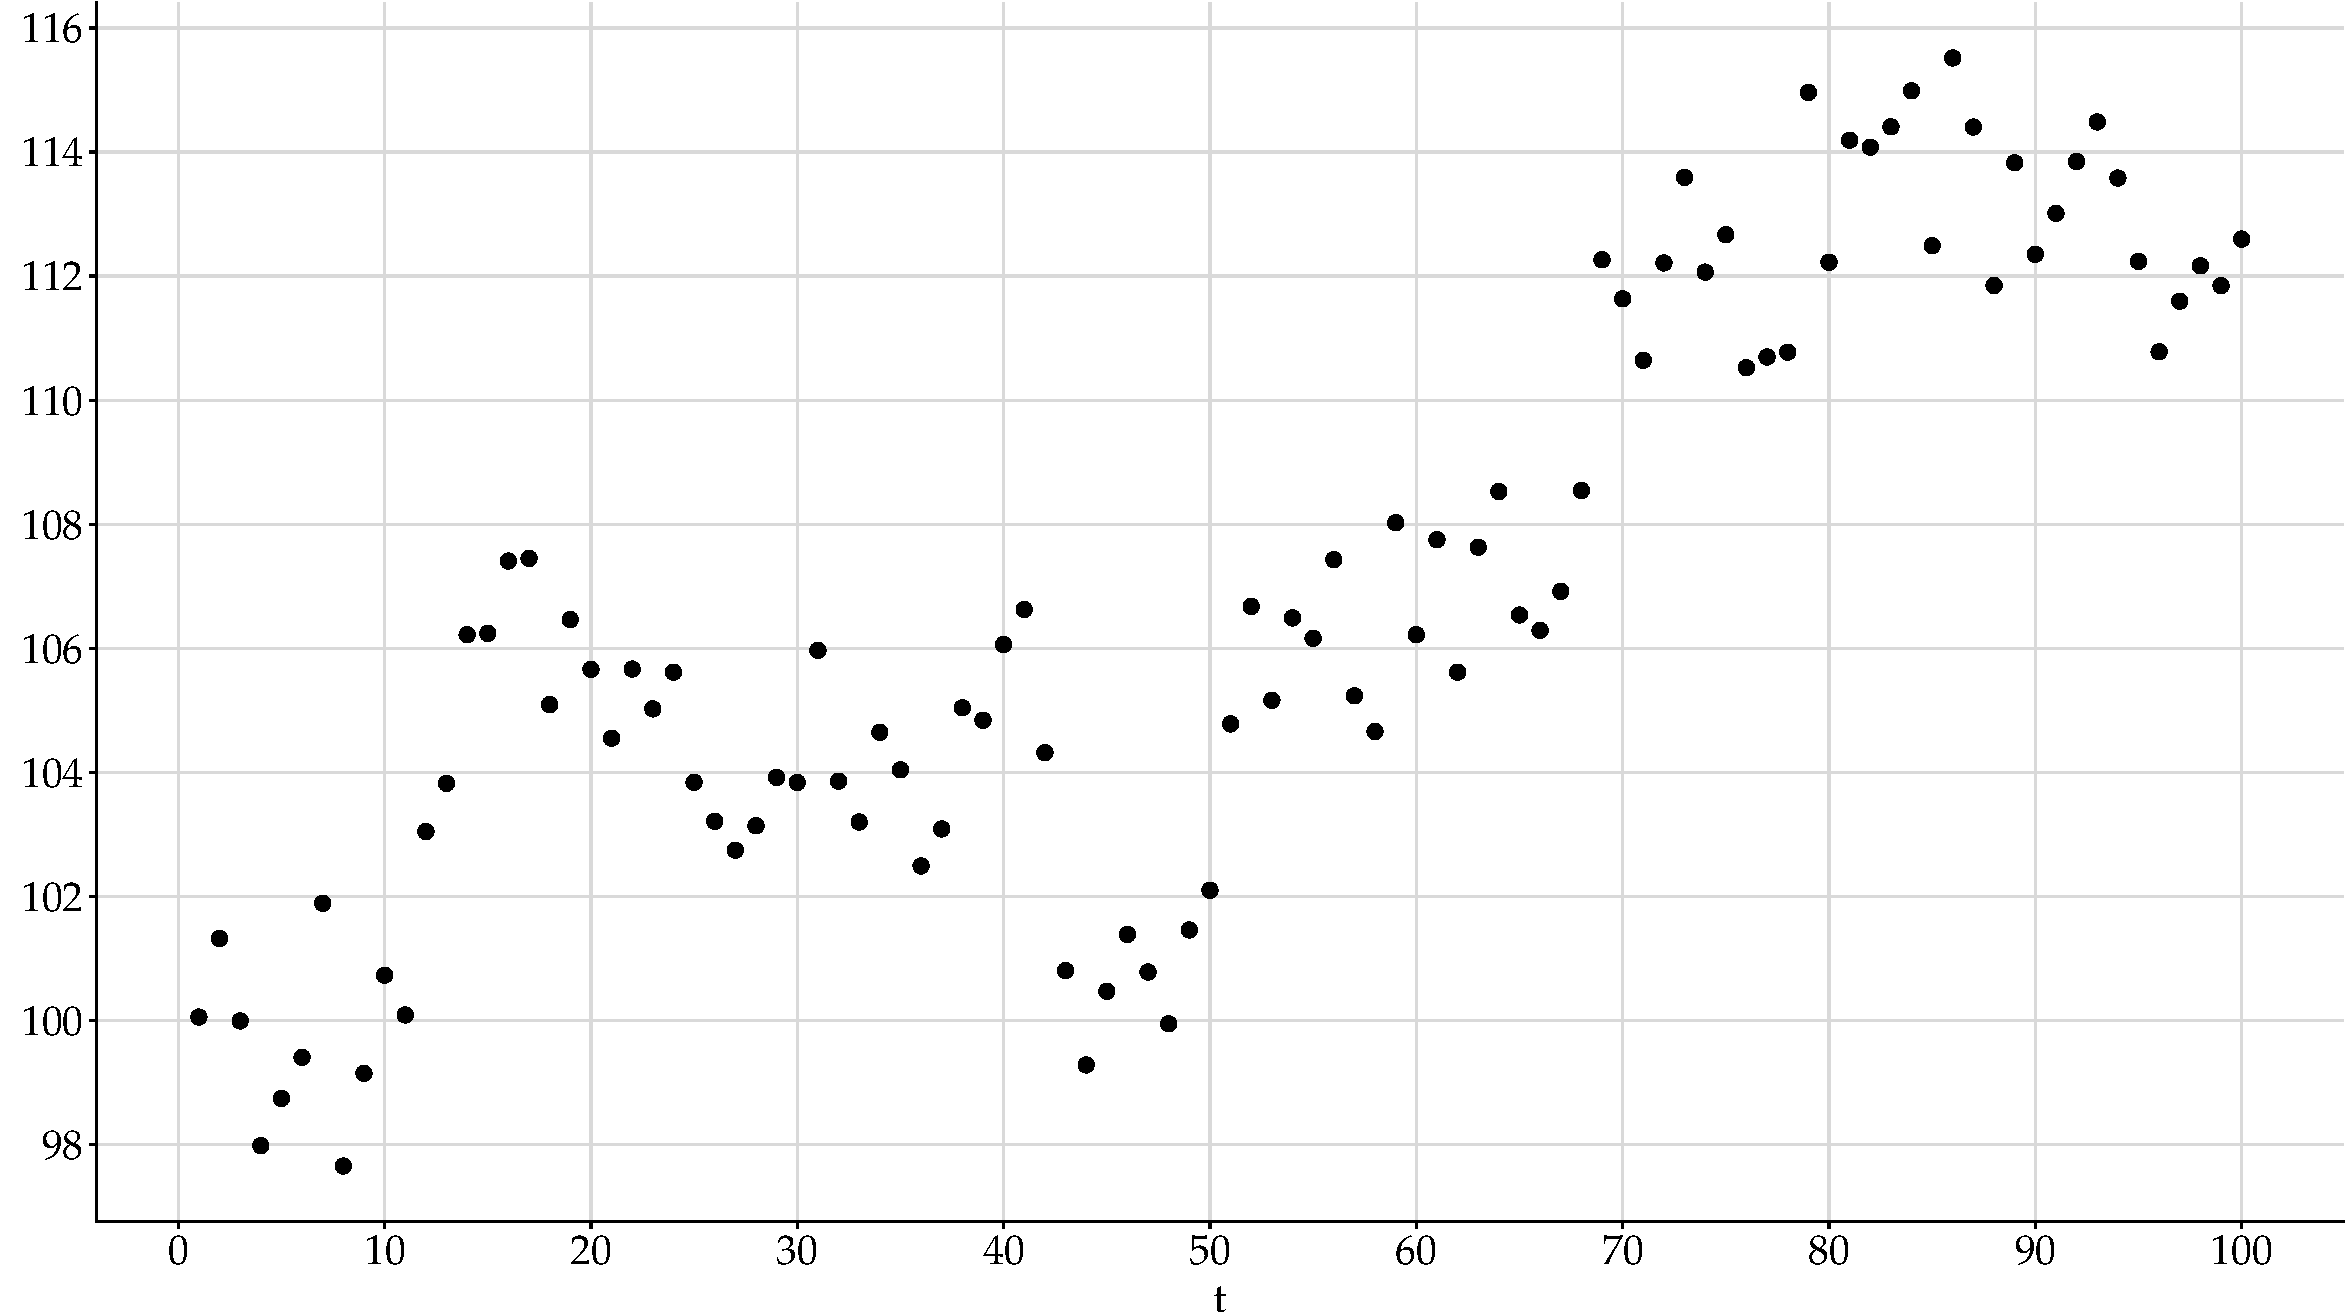
\includegraphics[width=0.9\linewidth]{pybats_detection_files/figure-latex/unnamed-chunk-2-1} 

}

\caption{Simulated data}\label{fig:unnamed-chunk-2}
\end{figure}

The Smoothing class allows you to perform a retrospective analysis for
\(\mathbf{Y}\), obtaining the distribution of
\((\boldsymbol{\theta}_{T-k} \vert D_T)\), for \(k \geq 1\), the k-step
smoothed distribution for the state vector at time \(T\), which is
analogous to the k-step ahead forecast distribution
\((\boldsymbol{\theta}_{t+k}\vert D_t)\).

To use Smoothing, first it is necessary to define the model components
with prior values, which is done with the \texttt{dlm} class available
in the \texttt{pybats} package. In this case, it was considered a DLM
with level and growth. The prior vector and covariances are defined by
\(\mathbf{a}\) and \(\mathbf{R}\). Lastly, the discount factor denoted
by \texttt{deltrend} is a constant in the interval {[}0, 1{]}, which is
used to coordinate the adaptive capacity of predictions with increasing
variance of model components.

\begin{Shaded}
\begin{Highlighting}[]
\OperatorTok{\textgreater{}\textgreater{}\textgreater{}} \CommentTok{\# Define model components}
\OperatorTok{\textgreater{}\textgreater{}\textgreater{}}\NormalTok{ a }\OperatorTok{=}\NormalTok{ np.array([}\DecValTok{100}\NormalTok{, }\DecValTok{0}\NormalTok{])}
\OperatorTok{\textgreater{}\textgreater{}\textgreater{}}\NormalTok{ R }\OperatorTok{=}\NormalTok{ np.eye(}\DecValTok{2}\NormalTok{)}
\OperatorTok{\textgreater{}\textgreater{}\textgreater{}}\NormalTok{ np.fill\_diagonal(R, val}\OperatorTok{=}\DecValTok{1}\NormalTok{)}
\OperatorTok{\textgreater{}\textgreater{}\textgreater{}}\NormalTok{ mod }\OperatorTok{=}\NormalTok{ dlm(a, R, ntrend}\OperatorTok{=}\DecValTok{2}\NormalTok{, deltrend}\OperatorTok{=}\FloatTok{.95}\NormalTok{)}
\end{Highlighting}
\end{Shaded}

Given this, the method \texttt{.fit} will initialize the model and the
loop forecast, observe and update begin. The prior and posterior moments
\((\mathbf{a}_t, \mathbf{m}_t, \mathbf{C}_t, \mathbf{R}_t)\) will be
computed for all \(t\) and saved. Subsequently, these moments will be
used to obtain the moments for
\((\boldsymbol{\theta}_{T-k} \vert D_T)\), recursively with
\(k \geq 1\), and denoted by
\((\mathbf{a}_T(-k), \mathbf{m}_T(-k), \mathbf{C}_T(-k), \mathbf{R}_T(-k))\).

\begin{Shaded}
\begin{Highlighting}[]
\OperatorTok{\textgreater{}\textgreater{}\textgreater{}} \CommentTok{\# Fit with monitoring}
\OperatorTok{\textgreater{}\textgreater{}\textgreater{}}\NormalTok{ smooth }\OperatorTok{=}\NormalTok{ Smoothing(mod}\OperatorTok{=}\NormalTok{mod)}
\OperatorTok{\textgreater{}\textgreater{}\textgreater{}}\NormalTok{ smooth\_fit }\OperatorTok{=}\NormalTok{ smooth.fit(y}\OperatorTok{=}\NormalTok{y)}
\end{Highlighting}
\end{Shaded}

This will return a dictionary with moments for: smoothed and filtered
predictive distributions and for the posterior distributions of the
model components. Each one can be obtained using the respective key

\begin{Shaded}
\begin{Highlighting}[]
\OperatorTok{\textgreater{}\textgreater{}\textgreater{}}\NormalTok{ smooth\_fit.get(}\StringTok{\textquotesingle{}smooth\textquotesingle{}}\NormalTok{).get(}\StringTok{\textquotesingle{}predictive\textquotesingle{}}\NormalTok{)}
\end{Highlighting}
\end{Shaded}

\begin{Shaded}
\begin{Highlighting}[]
\OperatorTok{\textgreater{}\textgreater{}\textgreater{}}\NormalTok{ smooth\_fit.get(}\StringTok{\textquotesingle{}smooth\textquotesingle{}}\NormalTok{).get(}\StringTok{\textquotesingle{}posterior\textquotesingle{}}\NormalTok{)}
\end{Highlighting}
\end{Shaded}

\begin{Shaded}
\begin{Highlighting}[]
\OperatorTok{\textgreater{}\textgreater{}\textgreater{}}\NormalTok{ smooth\_fit.get(}\StringTok{\textquotesingle{}filter\textquotesingle{}}\NormalTok{).get(}\StringTok{\textquotesingle{}predictive\textquotesingle{}}\NormalTok{)}
\end{Highlighting}
\end{Shaded}

\begin{Shaded}
\begin{Highlighting}[]
\OperatorTok{\textgreater{}\textgreater{}\textgreater{}}\NormalTok{ smooth\_fit.get(}\StringTok{\textquotesingle{}filter\textquotesingle{}}\NormalTok{).get(}\StringTok{\textquotesingle{}posterior\textquotesingle{}}\NormalTok{)}
\end{Highlighting}
\end{Shaded}

Below the results for the predictive and posterior smoothed
distributions

\hypertarget{smoothed-predictive}{%
\subsection{smoothed predictive}\label{smoothed-predictive}}

The results for the smoothed predictive distribution consists of:
\(f_T(-k), q_T(-k)\) and the bounds for the credible interval
(\texttt{ci\_lower}, \texttt{ci\_upper}). Given by

\[
f_T(-k) = \mathbf{F}^{'} \mathbf{a}_T(-k), \quad \quad q_T(-k) = \mathbf{F}^{'} \mathbf{R}_T(-k) \mathbf{F}
\] The credible interval is is obtained from the corresponding smoothed
distributions for the mean response of the series. Since \(V\) is
considered unknown, then

\[
(\mu_T(-k) \vert D_T) \sim T_{n_T}[f_T(-k), q_T(-k)]
\] For this simulated example, the results for the smoothed predictive
distribution for the mean response are

\begin{Shaded}
\begin{Highlighting}[]
\OperatorTok{\textgreater{}\textgreater{}\textgreater{}}\NormalTok{ smooth\_fit.get(}\StringTok{\textquotesingle{}smooth\textquotesingle{}}\NormalTok{).get(}\StringTok{\textquotesingle{}predictive\textquotesingle{}}\NormalTok{).}\BuiltInTok{round}\NormalTok{(}\DecValTok{2}\NormalTok{)}
\end{Highlighting}
\end{Shaded}

\begin{longtable}[]{@{}rrrrrr@{}}
\caption{Smothed predictive distribution results}\tabularnewline
\toprule
fk & qk & t & df & ci\_lower & ci\_upper \\
\midrule
\endfirsthead
\toprule
fk & qk & t & df & ci\_lower & ci\_upper \\
\midrule
\endhead
99.97 & 0.31 & 1 & 1 & 98.85 & 101.1 \\
100.07 & 0.27 & 2 & 2 & 99.05 & 101.1 \\
100.12 & 0.24 & 3 & 3 & 99.14 & 101.1 \\
100.20 & 0.23 & 4 & 4 & 99.24 & 101.2 \\
100.39 & 0.22 & 5 & 5 & 99.47 & 101.3 \\
100.64 & 0.21 & 6 & 6 & 99.73 & 101.6 \\
100.92 & 0.22 & 7 & 7 & 99.99 & 101.9 \\
101.16 & 0.21 & 8 & 8 & 100.24 & 102.1 \\
101.47 & 0.21 & 9 & 9 & 100.57 & 102.4 \\
101.83 & 0.21 & 10 & 10 & 100.93 & 102.7 \\
102.19 & 0.21 & 11 & 11 & 101.29 & 103.1 \\
102.57 & 0.22 & 12 & 12 & 101.65 & 103.5 \\
102.92 & 0.22 & 13 & 13 & 101.99 & 103.9 \\
103.24 & 0.23 & 14 & 14 & 102.29 & 104.2 \\
103.50 & 0.23 & 15 & 15 & 102.56 & 104.4 \\
103.70 & 0.22 & 16 & 16 & 102.77 & 104.6 \\
103.84 & 0.21 & 17 & 17 & 102.92 & 104.8 \\
103.92 & 0.21 & 18 & 18 & 103.01 & 104.8 \\
103.98 & 0.21 & 19 & 19 & 103.08 & 104.9 \\
104.01 & 0.20 & 20 & 20 & 103.12 & 104.9 \\
104.02 & 0.20 & 21 & 21 & 103.12 & 104.9 \\
104.02 & 0.20 & 22 & 22 & 103.13 & 104.9 \\
104.01 & 0.20 & 23 & 23 & 103.11 & 104.9 \\
103.99 & 0.21 & 24 & 24 & 103.09 & 104.9 \\
103.95 & 0.21 & 25 & 25 & 103.04 & 104.9 \\
103.92 & 0.21 & 26 & 26 & 103.01 & 104.8 \\
103.89 & 0.21 & 27 & 27 & 102.99 & 104.8 \\
103.89 & 0.21 & 28 & 28 & 102.98 & 104.8 \\
103.89 & 0.20 & 29 & 29 & 103.00 & 104.8 \\
103.90 & 0.20 & 30 & 30 & 103.01 & 104.8 \\
103.90 & 0.20 & 31 & 31 & 103.03 & 104.8 \\
103.90 & 0.19 & 32 & 32 & 103.03 & 104.8 \\
103.89 & 0.19 & 33 & 33 & 103.03 & 104.8 \\
103.90 & 0.19 & 34 & 34 & 103.04 & 104.8 \\
103.90 & 0.19 & 35 & 35 & 103.04 & 104.8 \\
103.91 & 0.19 & 36 & 36 & 103.05 & 104.8 \\
103.93 & 0.19 & 37 & 37 & 103.07 & 104.8 \\
103.96 & 0.18 & 38 & 38 & 103.11 & 104.8 \\
103.98 & 0.19 & 39 & 39 & 103.13 & 104.8 \\
104.01 & 0.19 & 40 & 40 & 103.15 & 104.9 \\
104.01 & 0.19 & 41 & 41 & 103.15 & 104.9 \\
104.01 & 0.19 & 42 & 42 & 103.14 & 104.9 \\
104.00 & 0.20 & 43 & 43 & 103.12 & 104.9 \\
104.02 & 0.20 & 44 & 44 & 103.13 & 104.9 \\
104.09 & 0.20 & 45 & 45 & 103.20 & 105.0 \\
104.18 & 0.20 & 46 & 46 & 103.29 & 105.1 \\
104.30 & 0.20 & 47 & 47 & 103.41 & 105.2 \\
104.44 & 0.20 & 48 & 48 & 103.56 & 105.3 \\
104.63 & 0.20 & 49 & 49 & 103.74 & 105.5 \\
104.83 & 0.20 & 50 & 50 & 103.95 & 105.7 \\
105.06 & 0.20 & 51 & 51 & 104.18 & 106.0 \\
105.29 & 0.20 & 52 & 52 & 104.40 & 106.2 \\
105.52 & 0.20 & 53 & 53 & 104.63 & 106.4 \\
105.74 & 0.20 & 54 & 54 & 104.86 & 106.6 \\
105.97 & 0.20 & 55 & 55 & 105.08 & 106.8 \\
106.19 & 0.20 & 56 & 56 & 105.31 & 107.1 \\
106.40 & 0.20 & 57 & 57 & 105.52 & 107.3 \\
106.63 & 0.20 & 58 & 58 & 105.75 & 107.5 \\
106.86 & 0.19 & 59 & 59 & 105.99 & 107.7 \\
107.10 & 0.19 & 60 & 60 & 106.22 & 108.0 \\
107.33 & 0.19 & 61 & 61 & 106.46 & 108.2 \\
107.57 & 0.19 & 62 & 62 & 106.70 & 108.4 \\
107.81 & 0.19 & 63 & 63 & 106.95 & 108.7 \\
108.06 & 0.19 & 64 & 64 & 107.20 & 108.9 \\
108.31 & 0.19 & 65 & 65 & 107.44 & 109.2 \\
108.57 & 0.19 & 66 & 66 & 107.70 & 109.4 \\
108.84 & 0.19 & 67 & 67 & 107.97 & 109.7 \\
109.12 & 0.19 & 68 & 68 & 108.25 & 110.0 \\
109.41 & 0.20 & 69 & 69 & 108.53 & 110.3 \\
109.67 & 0.20 & 70 & 70 & 108.80 & 110.5 \\
109.93 & 0.20 & 71 & 71 & 109.05 & 110.8 \\
110.18 & 0.20 & 72 & 72 & 109.30 & 111.1 \\
110.41 & 0.20 & 73 & 73 & 109.53 & 111.3 \\
110.63 & 0.20 & 74 & 74 & 109.75 & 111.5 \\
110.83 & 0.19 & 75 & 75 & 109.96 & 111.7 \\
111.02 & 0.19 & 76 & 76 & 110.15 & 111.9 \\
111.22 & 0.19 & 77 & 77 & 110.35 & 112.1 \\
111.42 & 0.19 & 78 & 78 & 110.55 & 112.3 \\
111.62 & 0.19 & 79 & 79 & 110.75 & 112.5 \\
111.80 & 0.19 & 80 & 80 & 110.93 & 112.7 \\
111.97 & 0.19 & 81 & 81 & 111.10 & 112.8 \\
112.13 & 0.19 & 82 & 82 & 111.26 & 113.0 \\
112.28 & 0.19 & 83 & 83 & 111.41 & 113.2 \\
112.42 & 0.20 & 84 & 84 & 111.54 & 113.3 \\
112.53 & 0.20 & 85 & 85 & 111.65 & 113.4 \\
112.65 & 0.20 & 86 & 86 & 111.76 & 113.5 \\
112.75 & 0.20 & 87 & 87 & 111.86 & 113.7 \\
112.84 & 0.21 & 88 & 88 & 111.94 & 113.8 \\
112.94 & 0.22 & 89 & 89 & 112.02 & 113.9 \\
113.03 & 0.22 & 90 & 90 & 112.09 & 114.0 \\
113.12 & 0.23 & 91 & 91 & 112.17 & 114.1 \\
113.22 & 0.24 & 92 & 92 & 112.24 & 114.2 \\
113.31 & 0.26 & 93 & 93 & 112.30 & 114.3 \\
113.39 & 0.28 & 94 & 94 & 112.35 & 114.4 \\
113.47 & 0.30 & 95 & 95 & 112.40 & 114.5 \\
113.56 & 0.32 & 96 & 96 & 112.44 & 114.7 \\
113.67 & 0.35 & 97 & 97 & 112.50 & 114.8 \\
113.78 & 0.38 & 98 & 98 & 112.56 & 115.0 \\
113.91 & 0.42 & 99 & 99 & 112.63 & 115.2 \\
114.05 & 0.46 & 100 & 100 & 112.70 & 115.4 \\
\bottomrule
\end{longtable}

as for the filtered distribution

\begin{Shaded}
\begin{Highlighting}[]
\OperatorTok{\textgreater{}\textgreater{}\textgreater{}}\NormalTok{ smooth\_fit.get(}\StringTok{\textquotesingle{}smooth\textquotesingle{}}\NormalTok{).get(}\StringTok{\textquotesingle{}predictive\textquotesingle{}}\NormalTok{).}\BuiltInTok{round}\NormalTok{(}\DecValTok{2}\NormalTok{)}
\end{Highlighting}
\end{Shaded}

\begin{longtable}[]{@{}lrrrrr@{}}
\caption{Filtered predictive distribution results}\tabularnewline
\toprule
parameter & mean & variance & t & ci\_lower & ci\_upper \\
\midrule
\endfirsthead
\toprule
parameter & mean & variance & t & ci\_lower & ci\_upper \\
\midrule
\endhead
Intercept & 99.97 & 0.31 & 1 & 98.85 & 101.08 \\
Intercept & 100.07 & 0.27 & 2 & 99.05 & 101.10 \\
Intercept & 100.12 & 0.24 & 3 & 99.14 & 101.11 \\
Intercept & 100.20 & 0.23 & 4 & 99.24 & 101.16 \\
Intercept & 100.39 & 0.22 & 5 & 99.47 & 101.32 \\
Intercept & 100.64 & 0.21 & 6 & 99.73 & 101.56 \\
Intercept & 100.92 & 0.22 & 7 & 99.99 & 101.86 \\
Intercept & 101.16 & 0.21 & 8 & 100.24 & 102.08 \\
Intercept & 101.47 & 0.21 & 9 & 100.57 & 102.38 \\
Intercept & 101.83 & 0.21 & 10 & 100.93 & 102.73 \\
Intercept & 102.19 & 0.21 & 11 & 101.29 & 103.09 \\
Intercept & 102.57 & 0.22 & 12 & 101.65 & 103.49 \\
Intercept & 102.92 & 0.22 & 13 & 101.99 & 103.86 \\
Intercept & 103.24 & 0.23 & 14 & 102.29 & 104.19 \\
Intercept & 103.50 & 0.23 & 15 & 102.56 & 104.44 \\
Intercept & 103.70 & 0.22 & 16 & 102.77 & 104.63 \\
Intercept & 103.84 & 0.21 & 17 & 102.92 & 104.75 \\
Intercept & 103.92 & 0.21 & 18 & 103.01 & 104.83 \\
Intercept & 103.98 & 0.21 & 19 & 103.08 & 104.88 \\
Intercept & 104.01 & 0.20 & 20 & 103.12 & 104.91 \\
Intercept & 104.02 & 0.20 & 21 & 103.12 & 104.92 \\
Intercept & 104.02 & 0.20 & 22 & 103.13 & 104.92 \\
Intercept & 104.01 & 0.20 & 23 & 103.11 & 104.91 \\
Intercept & 103.99 & 0.21 & 24 & 103.09 & 104.89 \\
Intercept & 103.95 & 0.21 & 25 & 103.04 & 104.86 \\
Intercept & 103.92 & 0.21 & 26 & 103.01 & 104.83 \\
Intercept & 103.89 & 0.21 & 27 & 102.99 & 104.80 \\
Intercept & 103.89 & 0.21 & 28 & 102.98 & 104.79 \\
Intercept & 103.89 & 0.20 & 29 & 103.00 & 104.78 \\
Intercept & 103.90 & 0.20 & 30 & 103.01 & 104.78 \\
Intercept & 103.90 & 0.20 & 31 & 103.03 & 104.78 \\
Intercept & 103.90 & 0.19 & 32 & 103.03 & 104.77 \\
Intercept & 103.89 & 0.19 & 33 & 103.03 & 104.76 \\
Intercept & 103.90 & 0.19 & 34 & 103.04 & 104.76 \\
Intercept & 103.90 & 0.19 & 35 & 103.04 & 104.76 \\
Intercept & 103.91 & 0.19 & 36 & 103.05 & 104.76 \\
Intercept & 103.93 & 0.19 & 37 & 103.07 & 104.78 \\
Intercept & 103.96 & 0.18 & 38 & 103.11 & 104.81 \\
Intercept & 103.98 & 0.19 & 39 & 103.13 & 104.84 \\
Intercept & 104.01 & 0.19 & 40 & 103.15 & 104.86 \\
Intercept & 104.01 & 0.19 & 41 & 103.15 & 104.88 \\
Intercept & 104.01 & 0.19 & 42 & 103.14 & 104.88 \\
Intercept & 104.00 & 0.20 & 43 & 103.12 & 104.88 \\
Intercept & 104.02 & 0.20 & 44 & 103.13 & 104.91 \\
Intercept & 104.09 & 0.20 & 45 & 103.20 & 104.98 \\
Intercept & 104.18 & 0.20 & 46 & 103.29 & 105.07 \\
Intercept & 104.30 & 0.20 & 47 & 103.41 & 105.19 \\
Intercept & 104.44 & 0.20 & 48 & 103.56 & 105.33 \\
Intercept & 104.63 & 0.20 & 49 & 103.74 & 105.51 \\
Intercept & 104.83 & 0.20 & 50 & 103.95 & 105.72 \\
Intercept & 105.06 & 0.20 & 51 & 104.18 & 105.95 \\
Intercept & 105.29 & 0.20 & 52 & 104.40 & 106.18 \\
Intercept & 105.52 & 0.20 & 53 & 104.63 & 106.40 \\
Intercept & 105.74 & 0.20 & 54 & 104.86 & 106.63 \\
Intercept & 105.97 & 0.20 & 55 & 105.08 & 106.85 \\
Intercept & 106.19 & 0.20 & 56 & 105.31 & 107.07 \\
Intercept & 106.40 & 0.20 & 57 & 105.52 & 107.28 \\
Intercept & 106.63 & 0.20 & 58 & 105.75 & 107.50 \\
Intercept & 106.86 & 0.19 & 59 & 105.99 & 107.74 \\
Intercept & 107.10 & 0.19 & 60 & 106.22 & 107.97 \\
Intercept & 107.33 & 0.19 & 61 & 106.46 & 108.20 \\
Intercept & 107.57 & 0.19 & 62 & 106.70 & 108.44 \\
Intercept & 107.81 & 0.19 & 63 & 106.95 & 108.68 \\
Intercept & 108.06 & 0.19 & 64 & 107.20 & 108.93 \\
Intercept & 108.31 & 0.19 & 65 & 107.44 & 109.18 \\
Intercept & 108.57 & 0.19 & 66 & 107.70 & 109.43 \\
Intercept & 108.84 & 0.19 & 67 & 107.97 & 109.71 \\
Intercept & 109.12 & 0.19 & 68 & 108.25 & 109.99 \\
Intercept & 109.41 & 0.20 & 69 & 108.53 & 110.28 \\
Intercept & 109.67 & 0.20 & 70 & 108.80 & 110.55 \\
Intercept & 109.93 & 0.20 & 71 & 109.05 & 110.81 \\
Intercept & 110.18 & 0.20 & 72 & 109.30 & 111.06 \\
Intercept & 110.41 & 0.20 & 73 & 109.53 & 111.29 \\
Intercept & 110.63 & 0.20 & 74 & 109.75 & 111.50 \\
Intercept & 110.83 & 0.19 & 75 & 109.96 & 111.71 \\
Intercept & 111.02 & 0.19 & 76 & 110.15 & 111.90 \\
Intercept & 111.22 & 0.19 & 77 & 110.35 & 112.09 \\
Intercept & 111.42 & 0.19 & 78 & 110.55 & 112.29 \\
Intercept & 111.62 & 0.19 & 79 & 110.75 & 112.49 \\
Intercept & 111.80 & 0.19 & 80 & 110.93 & 112.67 \\
Intercept & 111.97 & 0.19 & 81 & 111.10 & 112.84 \\
Intercept & 112.13 & 0.19 & 82 & 111.26 & 113.00 \\
Intercept & 112.28 & 0.19 & 83 & 111.41 & 113.15 \\
Intercept & 112.42 & 0.20 & 84 & 111.54 & 113.29 \\
Intercept & 112.53 & 0.20 & 85 & 111.65 & 113.42 \\
Intercept & 112.65 & 0.20 & 86 & 111.76 & 113.54 \\
Intercept & 112.75 & 0.20 & 87 & 111.86 & 113.65 \\
Intercept & 112.84 & 0.21 & 88 & 111.94 & 113.75 \\
Intercept & 112.94 & 0.22 & 89 & 112.02 & 113.86 \\
Intercept & 113.03 & 0.22 & 90 & 112.09 & 113.97 \\
Intercept & 113.12 & 0.23 & 91 & 112.17 & 114.08 \\
Intercept & 113.22 & 0.24 & 92 & 112.24 & 114.20 \\
Intercept & 113.31 & 0.26 & 93 & 112.30 & 114.32 \\
Intercept & 113.39 & 0.28 & 94 & 112.35 & 114.43 \\
Intercept & 113.47 & 0.30 & 95 & 112.40 & 114.55 \\
Intercept & 113.56 & 0.32 & 96 & 112.44 & 114.68 \\
Intercept & 113.67 & 0.35 & 97 & 112.50 & 114.84 \\
Intercept & 113.78 & 0.38 & 98 & 112.56 & 115.01 \\
Intercept & 113.91 & 0.42 & 99 & 112.63 & 115.19 \\
Intercept & 114.05 & 0.46 & 100 & 112.70 & 115.39 \\
Local Slope & 0.11 & 0.06 & 1 & -0.38 & 0.59 \\
Local Slope & 0.11 & 0.04 & 2 & -0.28 & 0.50 \\
Local Slope & 0.09 & 0.02 & 3 & -0.21 & 0.39 \\
Local Slope & 0.09 & 0.02 & 4 & -0.17 & 0.35 \\
Local Slope & 0.12 & 0.01 & 5 & -0.09 & 0.34 \\
Local Slope & 0.16 & 0.01 & 6 & -0.04 & 0.35 \\
Local Slope & 0.18 & 0.01 & 7 & -0.01 & 0.37 \\
Local Slope & 0.19 & 0.01 & 8 & 0.02 & 0.36 \\
Local Slope & 0.21 & 0.01 & 9 & 0.05 & 0.36 \\
Local Slope & 0.22 & 0.01 & 10 & 0.08 & 0.37 \\
Local Slope & 0.24 & 0.00 & 11 & 0.10 & 0.38 \\
Local Slope & 0.25 & 0.00 & 12 & 0.12 & 0.39 \\
Local Slope & 0.26 & 0.00 & 13 & 0.13 & 0.39 \\
Local Slope & 0.26 & 0.00 & 14 & 0.13 & 0.38 \\
Local Slope & 0.25 & 0.00 & 15 & 0.14 & 0.37 \\
Local Slope & 0.24 & 0.00 & 16 & 0.13 & 0.35 \\
Local Slope & 0.23 & 0.00 & 17 & 0.13 & 0.33 \\
Local Slope & 0.21 & 0.00 & 18 & 0.11 & 0.31 \\
Local Slope & 0.20 & 0.00 & 19 & 0.10 & 0.29 \\
Local Slope & 0.18 & 0.00 & 20 & 0.09 & 0.27 \\
Local Slope & 0.16 & 0.00 & 21 & 0.08 & 0.25 \\
Local Slope & 0.15 & 0.00 & 22 & 0.07 & 0.24 \\
Local Slope & 0.14 & 0.00 & 23 & 0.06 & 0.22 \\
Local Slope & 0.13 & 0.00 & 24 & 0.05 & 0.21 \\
Local Slope & 0.11 & 0.00 & 25 & 0.04 & 0.19 \\
Local Slope & 0.11 & 0.00 & 26 & 0.03 & 0.18 \\
Local Slope & 0.10 & 0.00 & 27 & 0.02 & 0.17 \\
Local Slope & 0.09 & 0.00 & 28 & 0.02 & 0.16 \\
Local Slope & 0.09 & 0.00 & 29 & 0.02 & 0.16 \\
Local Slope & 0.08 & 0.00 & 30 & 0.02 & 0.15 \\
Local Slope & 0.08 & 0.00 & 31 & 0.01 & 0.14 \\
Local Slope & 0.08 & 0.00 & 32 & 0.01 & 0.14 \\
Local Slope & 0.07 & 0.00 & 33 & 0.01 & 0.13 \\
Local Slope & 0.07 & 0.00 & 34 & 0.01 & 0.13 \\
Local Slope & 0.07 & 0.00 & 35 & 0.01 & 0.13 \\
Local Slope & 0.07 & 0.00 & 36 & 0.01 & 0.12 \\
Local Slope & 0.06 & 0.00 & 37 & 0.01 & 0.12 \\
Local Slope & 0.06 & 0.00 & 38 & 0.01 & 0.12 \\
Local Slope & 0.06 & 0.00 & 39 & 0.01 & 0.12 \\
Local Slope & 0.06 & 0.00 & 40 & 0.01 & 0.12 \\
Local Slope & 0.06 & 0.00 & 41 & 0.01 & 0.12 \\
Local Slope & 0.06 & 0.00 & 42 & 0.01 & 0.11 \\
Local Slope & 0.06 & 0.00 & 43 & 0.01 & 0.11 \\
Local Slope & 0.06 & 0.00 & 44 & 0.01 & 0.11 \\
Local Slope & 0.06 & 0.00 & 45 & 0.01 & 0.11 \\
Local Slope & 0.06 & 0.00 & 46 & 0.01 & 0.12 \\
Local Slope & 0.07 & 0.00 & 47 & 0.02 & 0.12 \\
Local Slope & 0.07 & 0.00 & 48 & 0.02 & 0.12 \\
Local Slope & 0.08 & 0.00 & 49 & 0.03 & 0.13 \\
Local Slope & 0.09 & 0.00 & 50 & 0.04 & 0.14 \\
Local Slope & 0.09 & 0.00 & 51 & 0.04 & 0.14 \\
Local Slope & 0.10 & 0.00 & 52 & 0.05 & 0.15 \\
Local Slope & 0.11 & 0.00 & 53 & 0.06 & 0.15 \\
Local Slope & 0.11 & 0.00 & 54 & 0.06 & 0.16 \\
Local Slope & 0.12 & 0.00 & 55 & 0.07 & 0.16 \\
Local Slope & 0.12 & 0.00 & 56 & 0.07 & 0.17 \\
Local Slope & 0.12 & 0.00 & 57 & 0.08 & 0.17 \\
Local Slope & 0.13 & 0.00 & 58 & 0.08 & 0.17 \\
Local Slope & 0.13 & 0.00 & 59 & 0.09 & 0.18 \\
Local Slope & 0.14 & 0.00 & 60 & 0.09 & 0.18 \\
Local Slope & 0.14 & 0.00 & 61 & 0.10 & 0.19 \\
Local Slope & 0.15 & 0.00 & 62 & 0.10 & 0.19 \\
Local Slope & 0.15 & 0.00 & 63 & 0.10 & 0.19 \\
Local Slope & 0.15 & 0.00 & 64 & 0.11 & 0.20 \\
Local Slope & 0.16 & 0.00 & 65 & 0.11 & 0.20 \\
Local Slope & 0.16 & 0.00 & 66 & 0.12 & 0.20 \\
Local Slope & 0.16 & 0.00 & 67 & 0.12 & 0.21 \\
Local Slope & 0.17 & 0.00 & 68 & 0.12 & 0.21 \\
Local Slope & 0.17 & 0.00 & 69 & 0.13 & 0.21 \\
Local Slope & 0.17 & 0.00 & 70 & 0.13 & 0.22 \\
Local Slope & 0.18 & 0.00 & 71 & 0.13 & 0.22 \\
Local Slope & 0.18 & 0.00 & 72 & 0.13 & 0.22 \\
Local Slope & 0.18 & 0.00 & 73 & 0.14 & 0.22 \\
Local Slope & 0.18 & 0.00 & 74 & 0.14 & 0.22 \\
Local Slope & 0.18 & 0.00 & 75 & 0.14 & 0.22 \\
Local Slope & 0.18 & 0.00 & 76 & 0.14 & 0.22 \\
Local Slope & 0.18 & 0.00 & 77 & 0.14 & 0.22 \\
Local Slope & 0.18 & 0.00 & 78 & 0.14 & 0.22 \\
Local Slope & 0.18 & 0.00 & 79 & 0.14 & 0.22 \\
Local Slope & 0.18 & 0.00 & 80 & 0.14 & 0.22 \\
Local Slope & 0.18 & 0.00 & 81 & 0.14 & 0.22 \\
Local Slope & 0.18 & 0.00 & 82 & 0.14 & 0.22 \\
Local Slope & 0.18 & 0.00 & 83 & 0.13 & 0.22 \\
Local Slope & 0.17 & 0.00 & 84 & 0.13 & 0.22 \\
Local Slope & 0.17 & 0.00 & 85 & 0.13 & 0.21 \\
Local Slope & 0.17 & 0.00 & 86 & 0.13 & 0.21 \\
Local Slope & 0.17 & 0.00 & 87 & 0.13 & 0.21 \\
Local Slope & 0.17 & 0.00 & 88 & 0.12 & 0.21 \\
Local Slope & 0.16 & 0.00 & 89 & 0.12 & 0.21 \\
Local Slope & 0.16 & 0.00 & 90 & 0.12 & 0.20 \\
Local Slope & 0.16 & 0.00 & 91 & 0.11 & 0.20 \\
Local Slope & 0.16 & 0.00 & 92 & 0.11 & 0.20 \\
Local Slope & 0.15 & 0.00 & 93 & 0.11 & 0.20 \\
Local Slope & 0.15 & 0.00 & 94 & 0.11 & 0.20 \\
Local Slope & 0.15 & 0.00 & 95 & 0.10 & 0.20 \\
Local Slope & 0.15 & 0.00 & 96 & 0.10 & 0.20 \\
Local Slope & 0.15 & 0.00 & 97 & 0.10 & 0.20 \\
Local Slope & 0.15 & 0.00 & 98 & 0.10 & 0.20 \\
Local Slope & 0.15 & 0.00 & 99 & 0.09 & 0.20 \\
Local Slope & 0.15 & 0.00 & 100 & 0.09 & 0.20 \\
\bottomrule
\end{longtable}

Plotting the filtered vs smoothed predictive distributions results is
possible to see difference, primarily in the length of the credible
interval.

\begin{figure}

{\centering 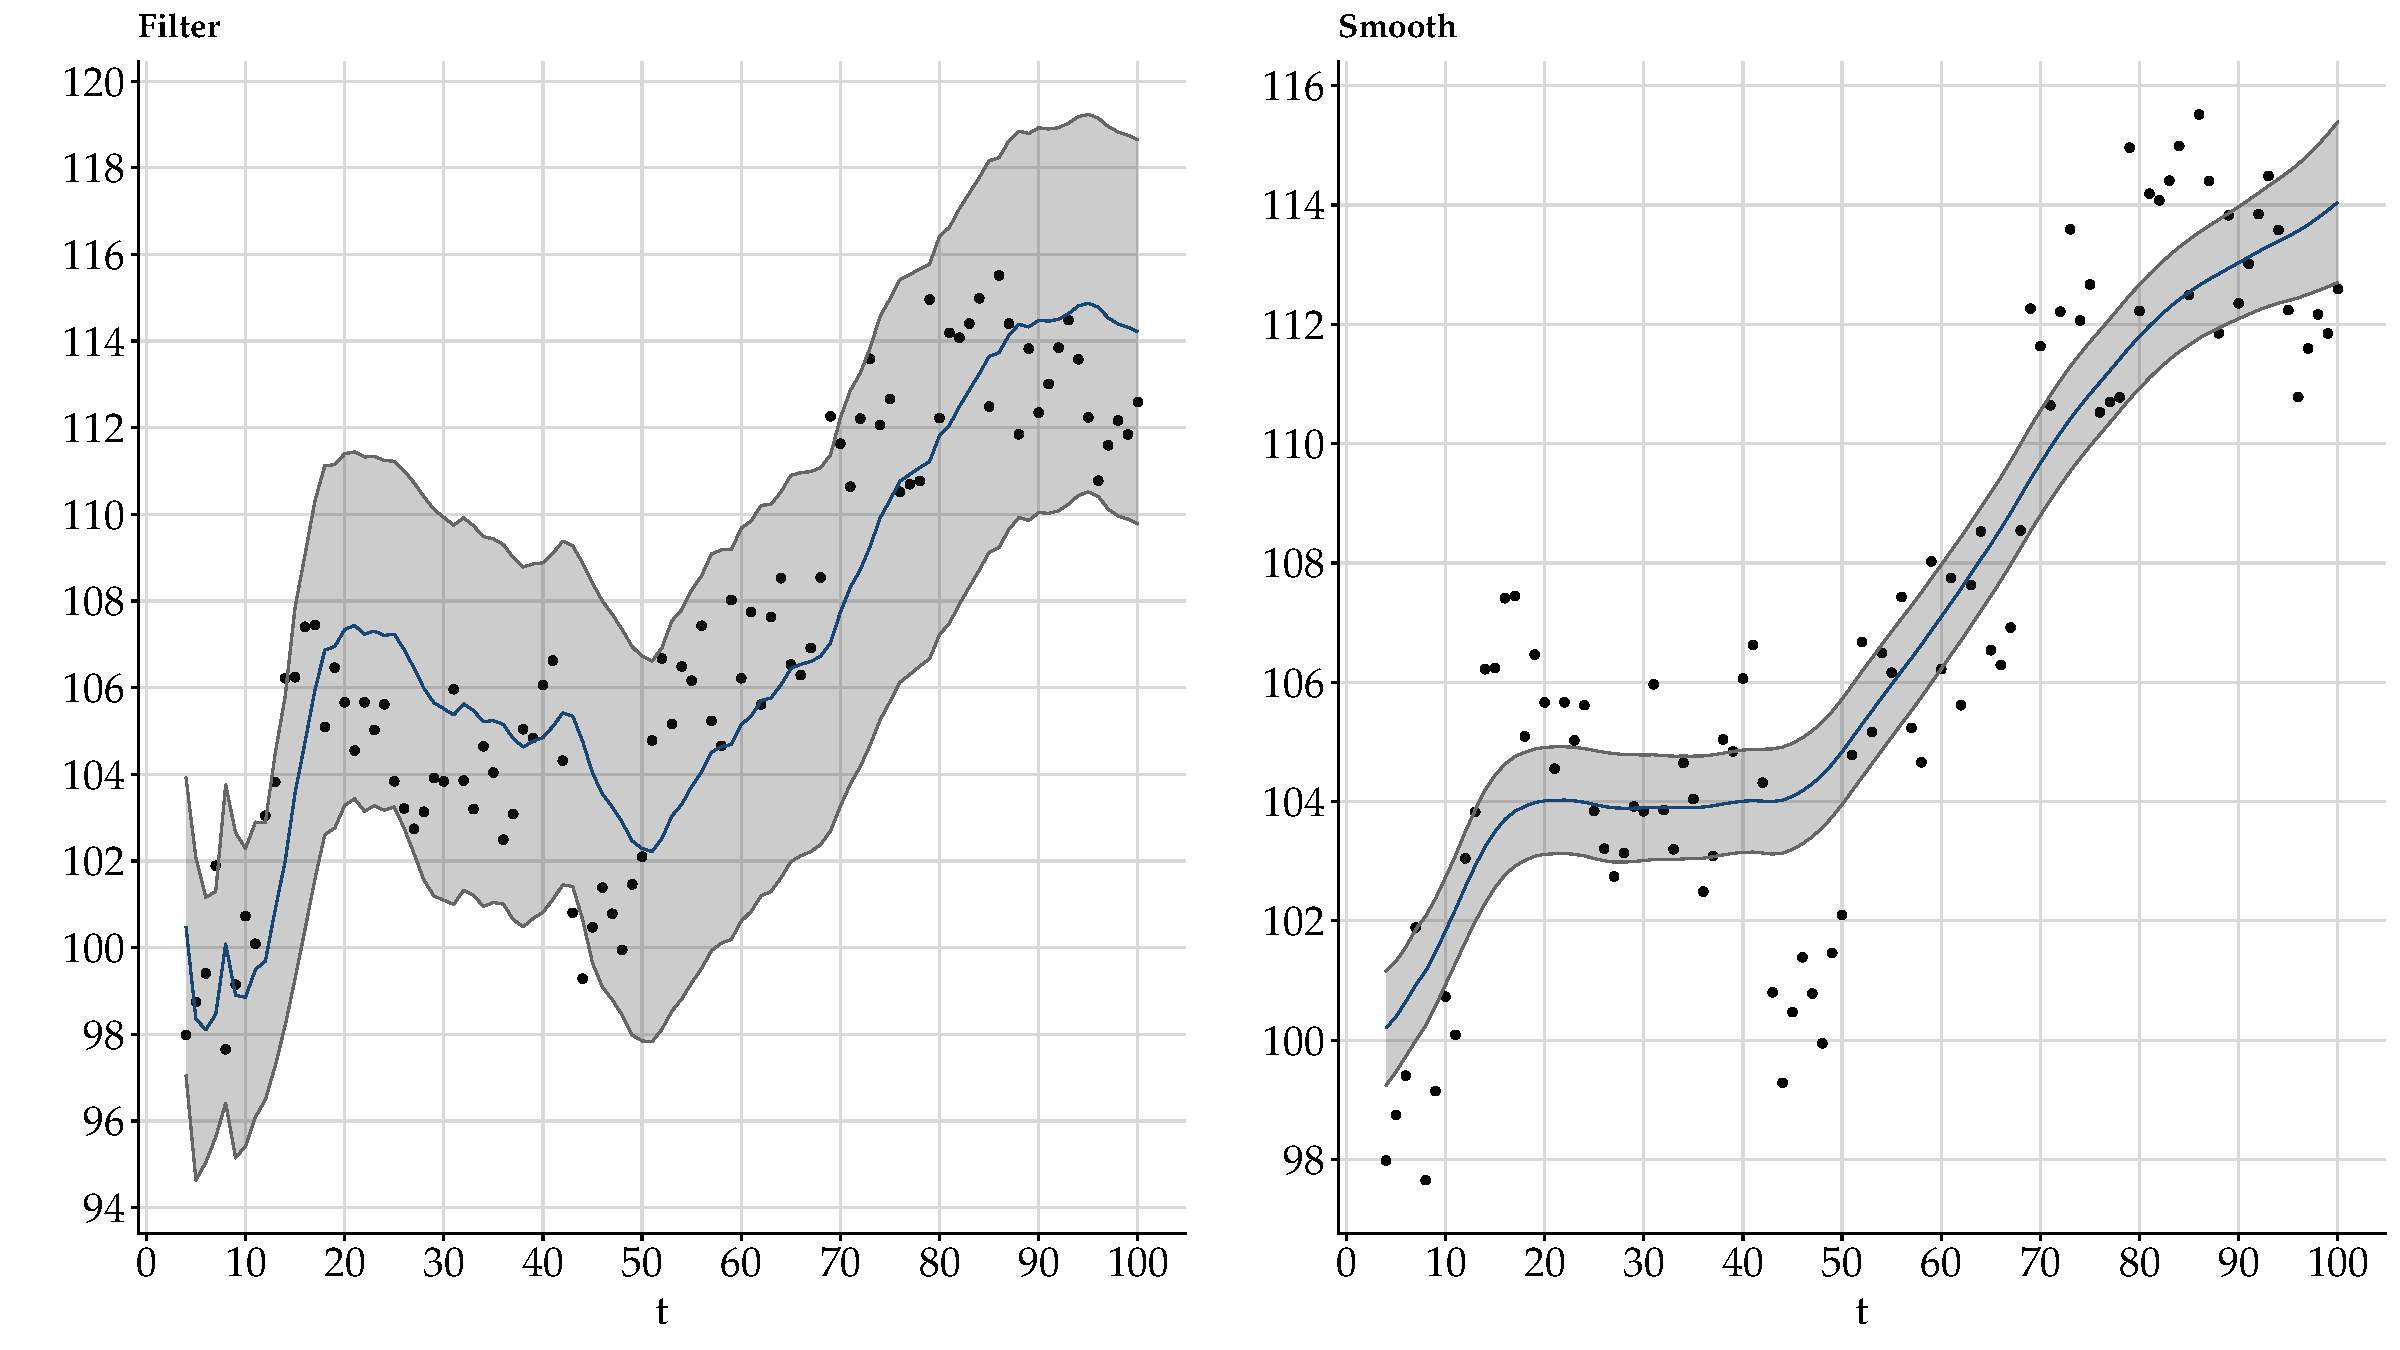
\includegraphics[width=0.9\linewidth]{pybats_detection_files/figure-latex/plots for smooth simulated example-1} 

}

\caption{Mean response for Filtered and Smoothed predictive distributions with $95\%$ credible intervals.}\label{fig:plots for smooth simulated example}
\end{figure}

\hypertarget{smoothed-posterior}{%
\subsection{smoothed posterior}\label{smoothed-posterior}}

The results for the posterior distributions are analogous, where

\begin{itemize}
\tightlist
\item
  parameter: Indicator for the respective state space parameter in
  \(\boldsymbol{\theta}\);
\item
  mean: The smoothed posterior distribution mean for time \(t=T-k\)
  (\(\mathbf{m}(-k)\));
\item
  variance: The smoothed posterior distribution variance for time \(t\)
  (\(\mathbf{C}(-k)\)).
\item
  credible interval (\texttt{ci\_lower}, \texttt{ci\_upper}): The
  credible interval obtained from the corresponding smoothed posterior
  distributions. Since \(V\) is considered unknown, then
\end{itemize}

\[
(\boldsymbol{\theta}_{T-k} \vert D_T) \sim T_{n_T}[\mathbf{a}_T(-k), \mathbf{R}_T(-k)].
\]

\begin{Shaded}
\begin{Highlighting}[]
\OperatorTok{\textgreater{}\textgreater{}\textgreater{}}\NormalTok{ smooth\_fit.get(}\StringTok{\textquotesingle{}smooth\textquotesingle{}}\NormalTok{).get(}\StringTok{\textquotesingle{}posterior\textquotesingle{}}\NormalTok{).}\BuiltInTok{round}\NormalTok{(}\DecValTok{2}\NormalTok{)}
\end{Highlighting}
\end{Shaded}

\begin{longtable}[]{@{}lrrrrr@{}}
\caption{Smothed posterior distribution results}\tabularnewline
\toprule
parameter & mean & variance & t & ci\_lower & ci\_upper \\
\midrule
\endfirsthead
\toprule
parameter & mean & variance & t & ci\_lower & ci\_upper \\
\midrule
\endhead
Intercept & 99.97 & 0.31 & 1 & 98.85 & 101.08 \\
Intercept & 100.07 & 0.27 & 2 & 99.05 & 101.10 \\
Intercept & 100.12 & 0.24 & 3 & 99.14 & 101.11 \\
Intercept & 100.20 & 0.23 & 4 & 99.24 & 101.16 \\
Intercept & 100.39 & 0.22 & 5 & 99.47 & 101.32 \\
Intercept & 100.64 & 0.21 & 6 & 99.73 & 101.56 \\
Intercept & 100.92 & 0.22 & 7 & 99.99 & 101.86 \\
Intercept & 101.16 & 0.21 & 8 & 100.24 & 102.08 \\
Intercept & 101.47 & 0.21 & 9 & 100.57 & 102.38 \\
Intercept & 101.83 & 0.21 & 10 & 100.93 & 102.73 \\
Intercept & 102.19 & 0.21 & 11 & 101.29 & 103.09 \\
Intercept & 102.57 & 0.22 & 12 & 101.65 & 103.49 \\
Intercept & 102.92 & 0.22 & 13 & 101.99 & 103.86 \\
Intercept & 103.24 & 0.23 & 14 & 102.29 & 104.19 \\
Intercept & 103.50 & 0.23 & 15 & 102.56 & 104.44 \\
Intercept & 103.70 & 0.22 & 16 & 102.77 & 104.63 \\
Intercept & 103.84 & 0.21 & 17 & 102.92 & 104.75 \\
Intercept & 103.92 & 0.21 & 18 & 103.01 & 104.83 \\
Intercept & 103.98 & 0.21 & 19 & 103.08 & 104.88 \\
Intercept & 104.01 & 0.20 & 20 & 103.12 & 104.91 \\
Intercept & 104.02 & 0.20 & 21 & 103.12 & 104.92 \\
Intercept & 104.02 & 0.20 & 22 & 103.13 & 104.92 \\
Intercept & 104.01 & 0.20 & 23 & 103.11 & 104.91 \\
Intercept & 103.99 & 0.21 & 24 & 103.09 & 104.89 \\
Intercept & 103.95 & 0.21 & 25 & 103.04 & 104.86 \\
Intercept & 103.92 & 0.21 & 26 & 103.01 & 104.83 \\
Intercept & 103.89 & 0.21 & 27 & 102.99 & 104.80 \\
Intercept & 103.89 & 0.21 & 28 & 102.98 & 104.79 \\
Intercept & 103.89 & 0.20 & 29 & 103.00 & 104.78 \\
Intercept & 103.90 & 0.20 & 30 & 103.01 & 104.78 \\
Intercept & 103.90 & 0.20 & 31 & 103.03 & 104.78 \\
Intercept & 103.90 & 0.19 & 32 & 103.03 & 104.77 \\
Intercept & 103.89 & 0.19 & 33 & 103.03 & 104.76 \\
Intercept & 103.90 & 0.19 & 34 & 103.04 & 104.76 \\
Intercept & 103.90 & 0.19 & 35 & 103.04 & 104.76 \\
Intercept & 103.91 & 0.19 & 36 & 103.05 & 104.76 \\
Intercept & 103.93 & 0.19 & 37 & 103.07 & 104.78 \\
Intercept & 103.96 & 0.18 & 38 & 103.11 & 104.81 \\
Intercept & 103.98 & 0.19 & 39 & 103.13 & 104.84 \\
Intercept & 104.01 & 0.19 & 40 & 103.15 & 104.86 \\
Intercept & 104.01 & 0.19 & 41 & 103.15 & 104.88 \\
Intercept & 104.01 & 0.19 & 42 & 103.14 & 104.88 \\
Intercept & 104.00 & 0.20 & 43 & 103.12 & 104.88 \\
Intercept & 104.02 & 0.20 & 44 & 103.13 & 104.91 \\
Intercept & 104.09 & 0.20 & 45 & 103.20 & 104.98 \\
Intercept & 104.18 & 0.20 & 46 & 103.29 & 105.07 \\
Intercept & 104.30 & 0.20 & 47 & 103.41 & 105.19 \\
Intercept & 104.44 & 0.20 & 48 & 103.56 & 105.33 \\
Intercept & 104.63 & 0.20 & 49 & 103.74 & 105.51 \\
Intercept & 104.83 & 0.20 & 50 & 103.95 & 105.72 \\
Intercept & 105.06 & 0.20 & 51 & 104.18 & 105.95 \\
Intercept & 105.29 & 0.20 & 52 & 104.40 & 106.18 \\
Intercept & 105.52 & 0.20 & 53 & 104.63 & 106.40 \\
Intercept & 105.74 & 0.20 & 54 & 104.86 & 106.63 \\
Intercept & 105.97 & 0.20 & 55 & 105.08 & 106.85 \\
Intercept & 106.19 & 0.20 & 56 & 105.31 & 107.07 \\
Intercept & 106.40 & 0.20 & 57 & 105.52 & 107.28 \\
Intercept & 106.63 & 0.20 & 58 & 105.75 & 107.50 \\
Intercept & 106.86 & 0.19 & 59 & 105.99 & 107.74 \\
Intercept & 107.10 & 0.19 & 60 & 106.22 & 107.97 \\
Intercept & 107.33 & 0.19 & 61 & 106.46 & 108.20 \\
Intercept & 107.57 & 0.19 & 62 & 106.70 & 108.44 \\
Intercept & 107.81 & 0.19 & 63 & 106.95 & 108.68 \\
Intercept & 108.06 & 0.19 & 64 & 107.20 & 108.93 \\
Intercept & 108.31 & 0.19 & 65 & 107.44 & 109.18 \\
Intercept & 108.57 & 0.19 & 66 & 107.70 & 109.43 \\
Intercept & 108.84 & 0.19 & 67 & 107.97 & 109.71 \\
Intercept & 109.12 & 0.19 & 68 & 108.25 & 109.99 \\
Intercept & 109.41 & 0.20 & 69 & 108.53 & 110.28 \\
Intercept & 109.67 & 0.20 & 70 & 108.80 & 110.55 \\
Intercept & 109.93 & 0.20 & 71 & 109.05 & 110.81 \\
Intercept & 110.18 & 0.20 & 72 & 109.30 & 111.06 \\
Intercept & 110.41 & 0.20 & 73 & 109.53 & 111.29 \\
Intercept & 110.63 & 0.20 & 74 & 109.75 & 111.50 \\
Intercept & 110.83 & 0.19 & 75 & 109.96 & 111.71 \\
Intercept & 111.02 & 0.19 & 76 & 110.15 & 111.90 \\
Intercept & 111.22 & 0.19 & 77 & 110.35 & 112.09 \\
Intercept & 111.42 & 0.19 & 78 & 110.55 & 112.29 \\
Intercept & 111.62 & 0.19 & 79 & 110.75 & 112.49 \\
Intercept & 111.80 & 0.19 & 80 & 110.93 & 112.67 \\
Intercept & 111.97 & 0.19 & 81 & 111.10 & 112.84 \\
Intercept & 112.13 & 0.19 & 82 & 111.26 & 113.00 \\
Intercept & 112.28 & 0.19 & 83 & 111.41 & 113.15 \\
Intercept & 112.42 & 0.20 & 84 & 111.54 & 113.29 \\
Intercept & 112.53 & 0.20 & 85 & 111.65 & 113.42 \\
Intercept & 112.65 & 0.20 & 86 & 111.76 & 113.54 \\
Intercept & 112.75 & 0.20 & 87 & 111.86 & 113.65 \\
Intercept & 112.84 & 0.21 & 88 & 111.94 & 113.75 \\
Intercept & 112.94 & 0.22 & 89 & 112.02 & 113.86 \\
Intercept & 113.03 & 0.22 & 90 & 112.09 & 113.97 \\
Intercept & 113.12 & 0.23 & 91 & 112.17 & 114.08 \\
Intercept & 113.22 & 0.24 & 92 & 112.24 & 114.20 \\
Intercept & 113.31 & 0.26 & 93 & 112.30 & 114.32 \\
Intercept & 113.39 & 0.28 & 94 & 112.35 & 114.43 \\
Intercept & 113.47 & 0.30 & 95 & 112.40 & 114.55 \\
Intercept & 113.56 & 0.32 & 96 & 112.44 & 114.68 \\
Intercept & 113.67 & 0.35 & 97 & 112.50 & 114.84 \\
Intercept & 113.78 & 0.38 & 98 & 112.56 & 115.01 \\
Intercept & 113.91 & 0.42 & 99 & 112.63 & 115.19 \\
Intercept & 114.05 & 0.46 & 100 & 112.70 & 115.39 \\
Local Slope & 0.11 & 0.06 & 1 & -0.38 & 0.59 \\
Local Slope & 0.11 & 0.04 & 2 & -0.28 & 0.50 \\
Local Slope & 0.09 & 0.02 & 3 & -0.21 & 0.39 \\
Local Slope & 0.09 & 0.02 & 4 & -0.17 & 0.35 \\
Local Slope & 0.12 & 0.01 & 5 & -0.09 & 0.34 \\
Local Slope & 0.16 & 0.01 & 6 & -0.04 & 0.35 \\
Local Slope & 0.18 & 0.01 & 7 & -0.01 & 0.37 \\
Local Slope & 0.19 & 0.01 & 8 & 0.02 & 0.36 \\
Local Slope & 0.21 & 0.01 & 9 & 0.05 & 0.36 \\
Local Slope & 0.22 & 0.01 & 10 & 0.08 & 0.37 \\
Local Slope & 0.24 & 0.00 & 11 & 0.10 & 0.38 \\
Local Slope & 0.25 & 0.00 & 12 & 0.12 & 0.39 \\
Local Slope & 0.26 & 0.00 & 13 & 0.13 & 0.39 \\
Local Slope & 0.26 & 0.00 & 14 & 0.13 & 0.38 \\
Local Slope & 0.25 & 0.00 & 15 & 0.14 & 0.37 \\
Local Slope & 0.24 & 0.00 & 16 & 0.13 & 0.35 \\
Local Slope & 0.23 & 0.00 & 17 & 0.13 & 0.33 \\
Local Slope & 0.21 & 0.00 & 18 & 0.11 & 0.31 \\
Local Slope & 0.20 & 0.00 & 19 & 0.10 & 0.29 \\
Local Slope & 0.18 & 0.00 & 20 & 0.09 & 0.27 \\
Local Slope & 0.16 & 0.00 & 21 & 0.08 & 0.25 \\
Local Slope & 0.15 & 0.00 & 22 & 0.07 & 0.24 \\
Local Slope & 0.14 & 0.00 & 23 & 0.06 & 0.22 \\
Local Slope & 0.13 & 0.00 & 24 & 0.05 & 0.21 \\
Local Slope & 0.11 & 0.00 & 25 & 0.04 & 0.19 \\
Local Slope & 0.11 & 0.00 & 26 & 0.03 & 0.18 \\
Local Slope & 0.10 & 0.00 & 27 & 0.02 & 0.17 \\
Local Slope & 0.09 & 0.00 & 28 & 0.02 & 0.16 \\
Local Slope & 0.09 & 0.00 & 29 & 0.02 & 0.16 \\
Local Slope & 0.08 & 0.00 & 30 & 0.02 & 0.15 \\
Local Slope & 0.08 & 0.00 & 31 & 0.01 & 0.14 \\
Local Slope & 0.08 & 0.00 & 32 & 0.01 & 0.14 \\
Local Slope & 0.07 & 0.00 & 33 & 0.01 & 0.13 \\
Local Slope & 0.07 & 0.00 & 34 & 0.01 & 0.13 \\
Local Slope & 0.07 & 0.00 & 35 & 0.01 & 0.13 \\
Local Slope & 0.07 & 0.00 & 36 & 0.01 & 0.12 \\
Local Slope & 0.06 & 0.00 & 37 & 0.01 & 0.12 \\
Local Slope & 0.06 & 0.00 & 38 & 0.01 & 0.12 \\
Local Slope & 0.06 & 0.00 & 39 & 0.01 & 0.12 \\
Local Slope & 0.06 & 0.00 & 40 & 0.01 & 0.12 \\
Local Slope & 0.06 & 0.00 & 41 & 0.01 & 0.12 \\
Local Slope & 0.06 & 0.00 & 42 & 0.01 & 0.11 \\
Local Slope & 0.06 & 0.00 & 43 & 0.01 & 0.11 \\
Local Slope & 0.06 & 0.00 & 44 & 0.01 & 0.11 \\
Local Slope & 0.06 & 0.00 & 45 & 0.01 & 0.11 \\
Local Slope & 0.06 & 0.00 & 46 & 0.01 & 0.12 \\
Local Slope & 0.07 & 0.00 & 47 & 0.02 & 0.12 \\
Local Slope & 0.07 & 0.00 & 48 & 0.02 & 0.12 \\
Local Slope & 0.08 & 0.00 & 49 & 0.03 & 0.13 \\
Local Slope & 0.09 & 0.00 & 50 & 0.04 & 0.14 \\
Local Slope & 0.09 & 0.00 & 51 & 0.04 & 0.14 \\
Local Slope & 0.10 & 0.00 & 52 & 0.05 & 0.15 \\
Local Slope & 0.11 & 0.00 & 53 & 0.06 & 0.15 \\
Local Slope & 0.11 & 0.00 & 54 & 0.06 & 0.16 \\
Local Slope & 0.12 & 0.00 & 55 & 0.07 & 0.16 \\
Local Slope & 0.12 & 0.00 & 56 & 0.07 & 0.17 \\
Local Slope & 0.12 & 0.00 & 57 & 0.08 & 0.17 \\
Local Slope & 0.13 & 0.00 & 58 & 0.08 & 0.17 \\
Local Slope & 0.13 & 0.00 & 59 & 0.09 & 0.18 \\
Local Slope & 0.14 & 0.00 & 60 & 0.09 & 0.18 \\
Local Slope & 0.14 & 0.00 & 61 & 0.10 & 0.19 \\
Local Slope & 0.15 & 0.00 & 62 & 0.10 & 0.19 \\
Local Slope & 0.15 & 0.00 & 63 & 0.10 & 0.19 \\
Local Slope & 0.15 & 0.00 & 64 & 0.11 & 0.20 \\
Local Slope & 0.16 & 0.00 & 65 & 0.11 & 0.20 \\
Local Slope & 0.16 & 0.00 & 66 & 0.12 & 0.20 \\
Local Slope & 0.16 & 0.00 & 67 & 0.12 & 0.21 \\
Local Slope & 0.17 & 0.00 & 68 & 0.12 & 0.21 \\
Local Slope & 0.17 & 0.00 & 69 & 0.13 & 0.21 \\
Local Slope & 0.17 & 0.00 & 70 & 0.13 & 0.22 \\
Local Slope & 0.18 & 0.00 & 71 & 0.13 & 0.22 \\
Local Slope & 0.18 & 0.00 & 72 & 0.13 & 0.22 \\
Local Slope & 0.18 & 0.00 & 73 & 0.14 & 0.22 \\
Local Slope & 0.18 & 0.00 & 74 & 0.14 & 0.22 \\
Local Slope & 0.18 & 0.00 & 75 & 0.14 & 0.22 \\
Local Slope & 0.18 & 0.00 & 76 & 0.14 & 0.22 \\
Local Slope & 0.18 & 0.00 & 77 & 0.14 & 0.22 \\
Local Slope & 0.18 & 0.00 & 78 & 0.14 & 0.22 \\
Local Slope & 0.18 & 0.00 & 79 & 0.14 & 0.22 \\
Local Slope & 0.18 & 0.00 & 80 & 0.14 & 0.22 \\
Local Slope & 0.18 & 0.00 & 81 & 0.14 & 0.22 \\
Local Slope & 0.18 & 0.00 & 82 & 0.14 & 0.22 \\
Local Slope & 0.18 & 0.00 & 83 & 0.13 & 0.22 \\
Local Slope & 0.17 & 0.00 & 84 & 0.13 & 0.22 \\
Local Slope & 0.17 & 0.00 & 85 & 0.13 & 0.21 \\
Local Slope & 0.17 & 0.00 & 86 & 0.13 & 0.21 \\
Local Slope & 0.17 & 0.00 & 87 & 0.13 & 0.21 \\
Local Slope & 0.17 & 0.00 & 88 & 0.12 & 0.21 \\
Local Slope & 0.16 & 0.00 & 89 & 0.12 & 0.21 \\
Local Slope & 0.16 & 0.00 & 90 & 0.12 & 0.20 \\
Local Slope & 0.16 & 0.00 & 91 & 0.11 & 0.20 \\
Local Slope & 0.16 & 0.00 & 92 & 0.11 & 0.20 \\
Local Slope & 0.15 & 0.00 & 93 & 0.11 & 0.20 \\
Local Slope & 0.15 & 0.00 & 94 & 0.11 & 0.20 \\
Local Slope & 0.15 & 0.00 & 95 & 0.10 & 0.20 \\
Local Slope & 0.15 & 0.00 & 96 & 0.10 & 0.20 \\
Local Slope & 0.15 & 0.00 & 97 & 0.10 & 0.20 \\
Local Slope & 0.15 & 0.00 & 98 & 0.10 & 0.20 \\
Local Slope & 0.15 & 0.00 & 99 & 0.09 & 0.20 \\
Local Slope & 0.15 & 0.00 & 100 & 0.09 & 0.20 \\
\bottomrule
\end{longtable}

As before we plot the results for filtered and smoothed distributions,
in this case for each state space parameter. As expected, the smoothed
posterior distributions show a less erratic behavior with shorter
credible intervals.

\begin{figure}

{\centering 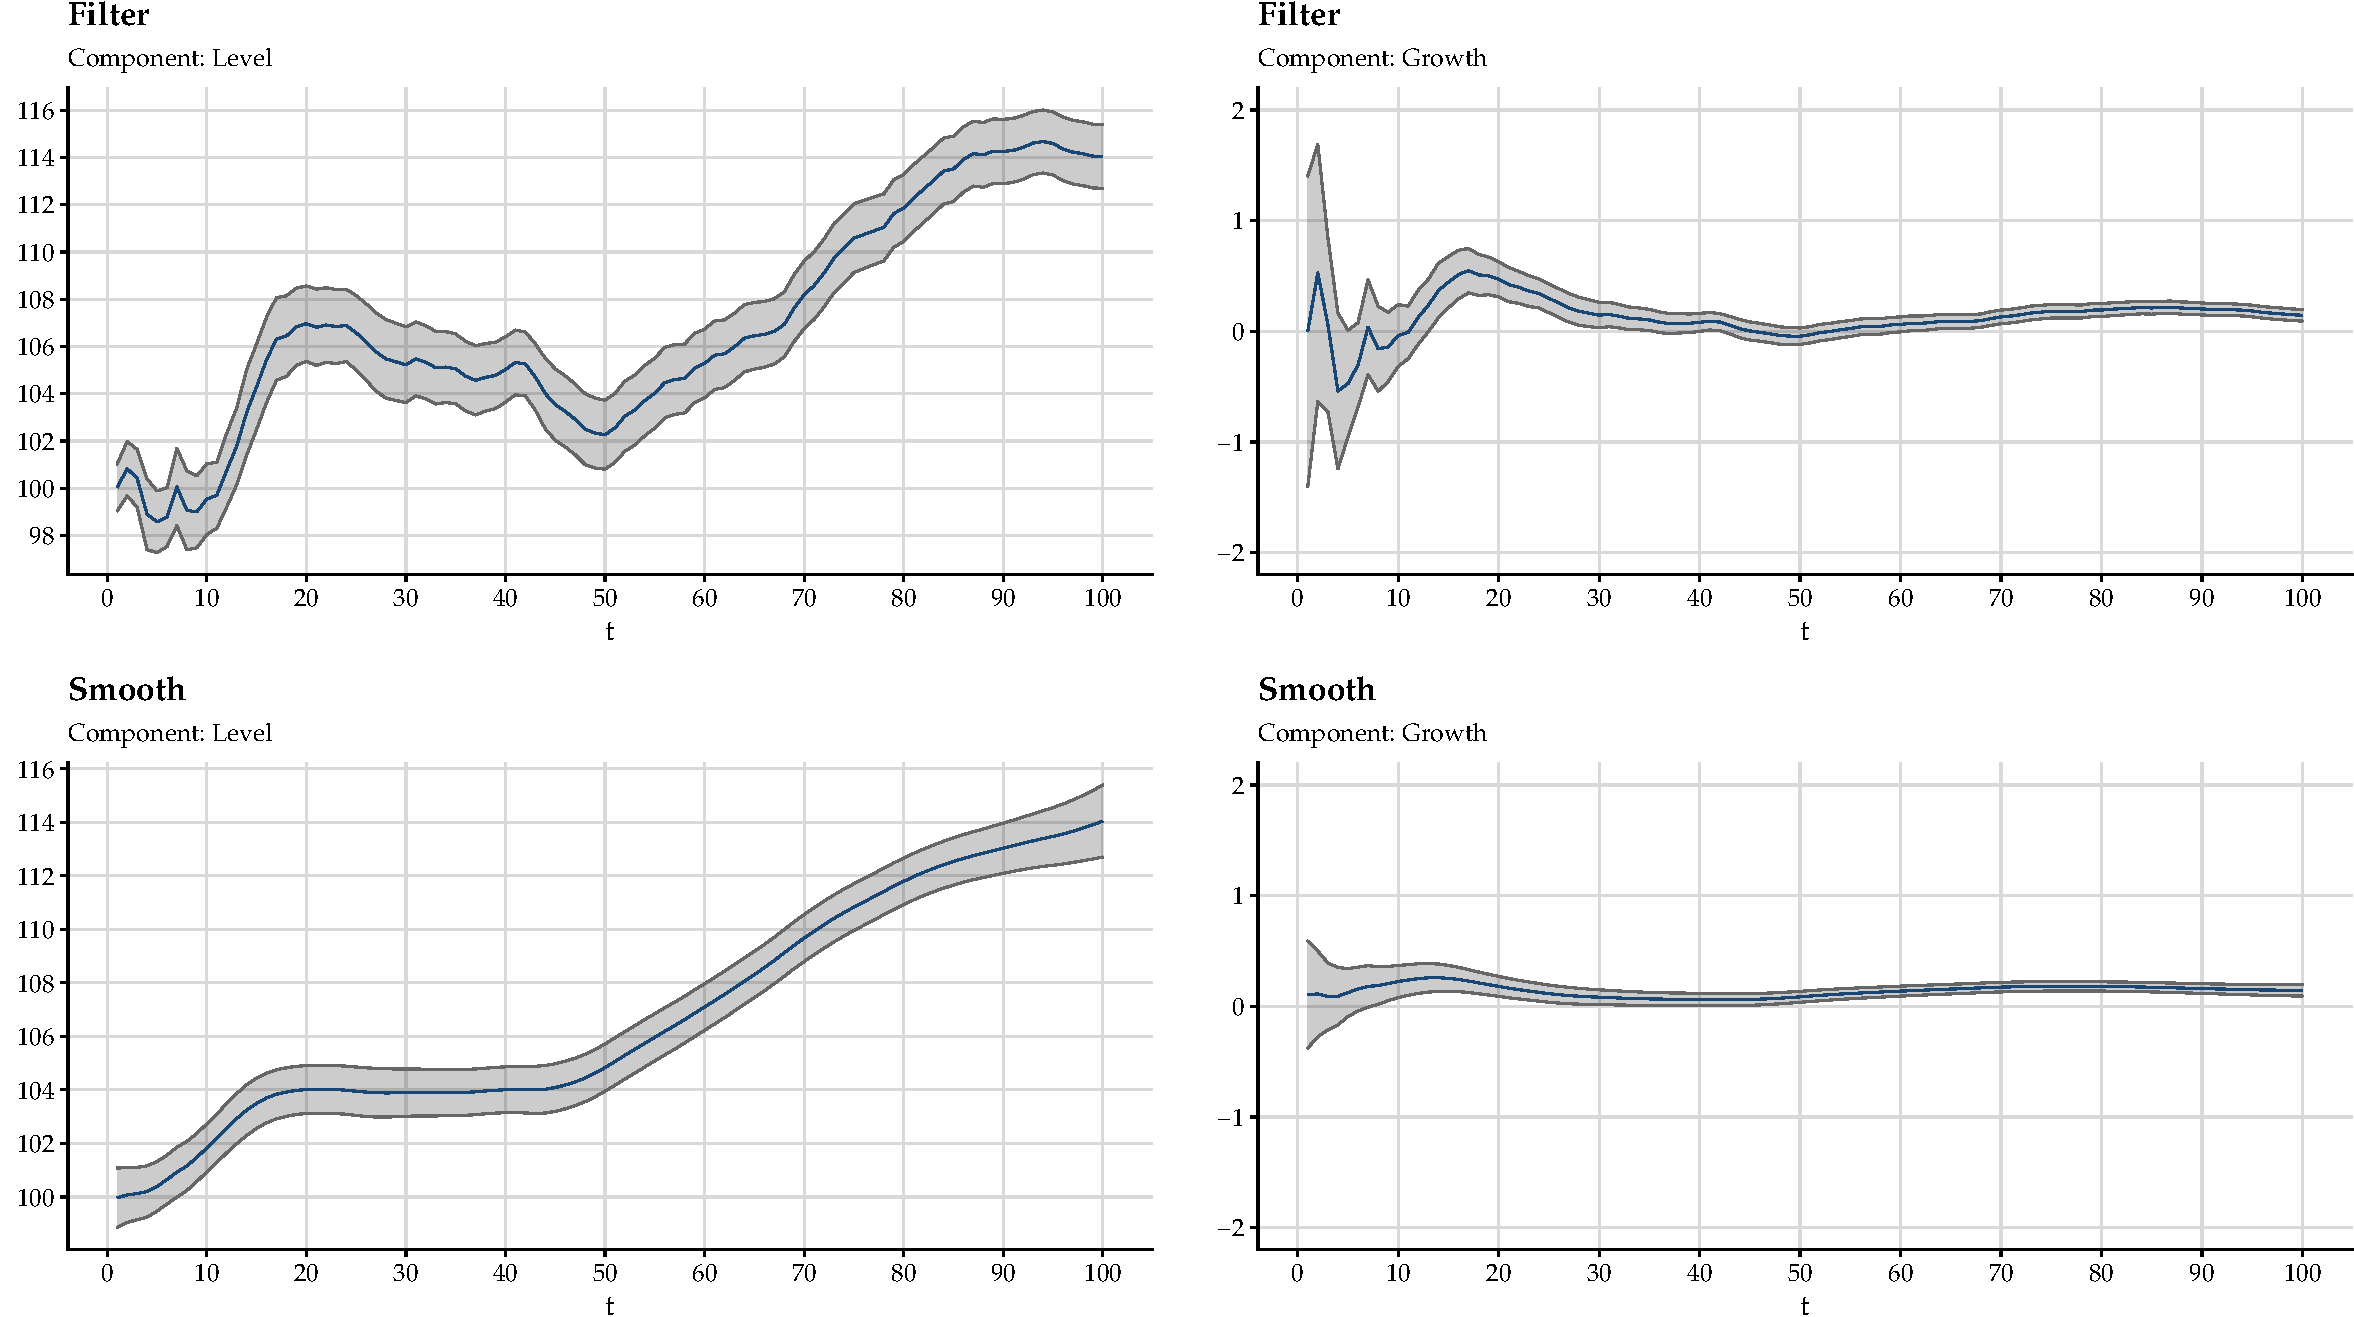
\includegraphics[width=0.9\linewidth]{pybats_detection_files/figure-latex/unnamed-chunk-13-1} 

}

\caption{Mean response for Filtered and Smoothed posterior distributions for each model component with $95\%$ credible intervals.}\label{fig:unnamed-chunk-13}
\end{figure}

\hypertarget{aplication-airpassangers-dataset}{%
\subsection{Aplication: AirPassangers
dataset}\label{aplication-airpassangers-dataset}}

Below is a practical example with the classic Box \& Jenkins airline
data, Monthly totals of international airline passengers (1949 to 1960).
This data has a clear multiplicative seasonality, using a linear model
(with additive seasonality) may be a naive approximation for this data.
But, just for the sake of comparison between filtered and smoothing we
stick with the linear model.

\begin{figure}

{\centering 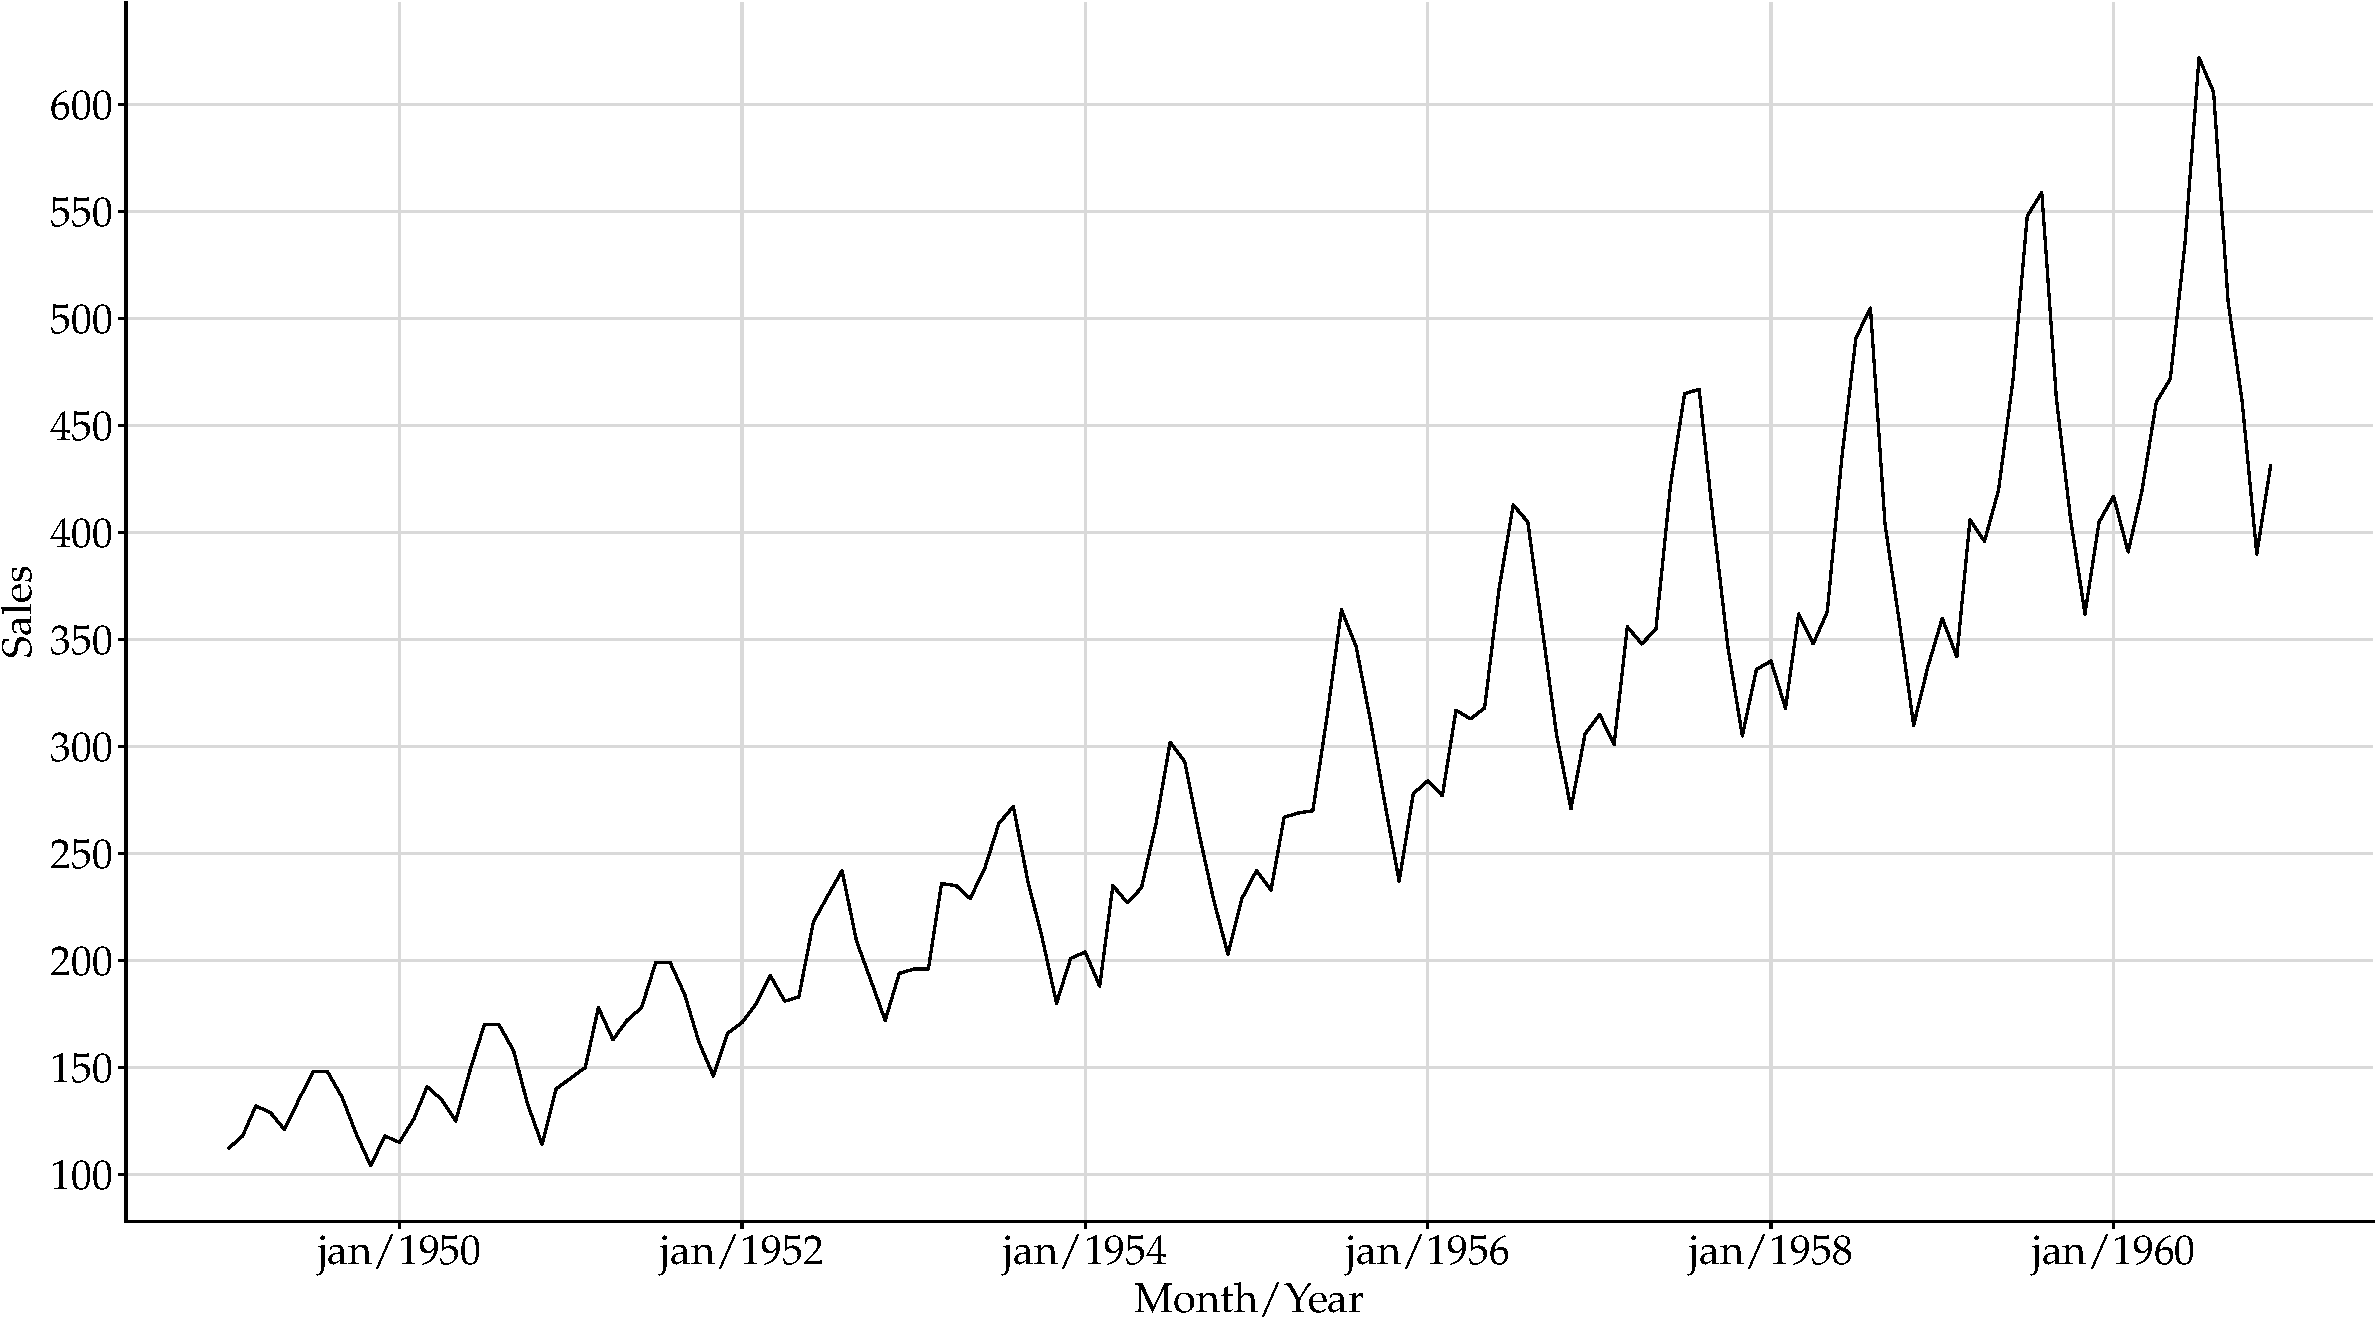
\includegraphics[width=0.9\linewidth]{pybats_detection_files/figure-latex/unnamed-chunk-14-1} 

}

\caption{Monthly totals of international airline passengers, 1949 to 1960.}\label{fig:unnamed-chunk-14}
\end{figure}

Using a normal DLM with three main components: Trend, Growth and
Seasonality. The seasonality is modeled using the Fourier form
representation, which depends on the parity of a period \(p\) and the
number of harmonics components. Formally, the \(\mathbf{r}^{th}\)
harmonic component is given by

\[
S_r(.) = a_r \cos(\alpha r) + b_r \sin(\alpha r), \quad r=1, \dots, h, \quad 
a_r = 2\pi/p, \quad h <= p /2 
\] Here it was specified a yearly seasonal effect with period \(p=12\)
and the first two harmonics. The discount factor for the level and
growth components is set to 0.95, and 0.98 for the seasonal components.
The results are plotted below.

\begin{Shaded}
\begin{Highlighting}[]
\OperatorTok{\textgreater{}\textgreater{}\textgreater{}}\NormalTok{ a }\OperatorTok{=}\NormalTok{ np.array([}\DecValTok{112}\NormalTok{, }\DecValTok{0}\NormalTok{, }\DecValTok{0}\NormalTok{, }\DecValTok{0}\NormalTok{, }\DecValTok{0}\NormalTok{, }\DecValTok{0}\NormalTok{])}
\OperatorTok{\textgreater{}\textgreater{}\textgreater{}}\NormalTok{ R }\OperatorTok{=}\NormalTok{ np.eye(}\DecValTok{6}\NormalTok{)}
\OperatorTok{\textgreater{}\textgreater{}\textgreater{}}\NormalTok{ np.fill\_diagonal(R, val}\OperatorTok{=}\DecValTok{100}\NormalTok{)}
\OperatorTok{\textgreater{}\textgreater{}\textgreater{}}\NormalTok{ mod }\OperatorTok{=}\NormalTok{ dlm(a, R, ntrend}\OperatorTok{=}\DecValTok{2}\NormalTok{, deltrend}\OperatorTok{=}\FloatTok{.95}\NormalTok{, delseas}\OperatorTok{=}\FloatTok{.98}\NormalTok{,}
\OperatorTok{\textgreater{}\textgreater{}\textgreater{}}\NormalTok{           seasPeriods}\OperatorTok{=}\NormalTok{[}\DecValTok{12}\NormalTok{], seasHarmComponents}\OperatorTok{=}\NormalTok{[[}\DecValTok{1}\NormalTok{, }\DecValTok{2}\NormalTok{]])}
\end{Highlighting}
\end{Shaded}

\begin{figure}

{\centering 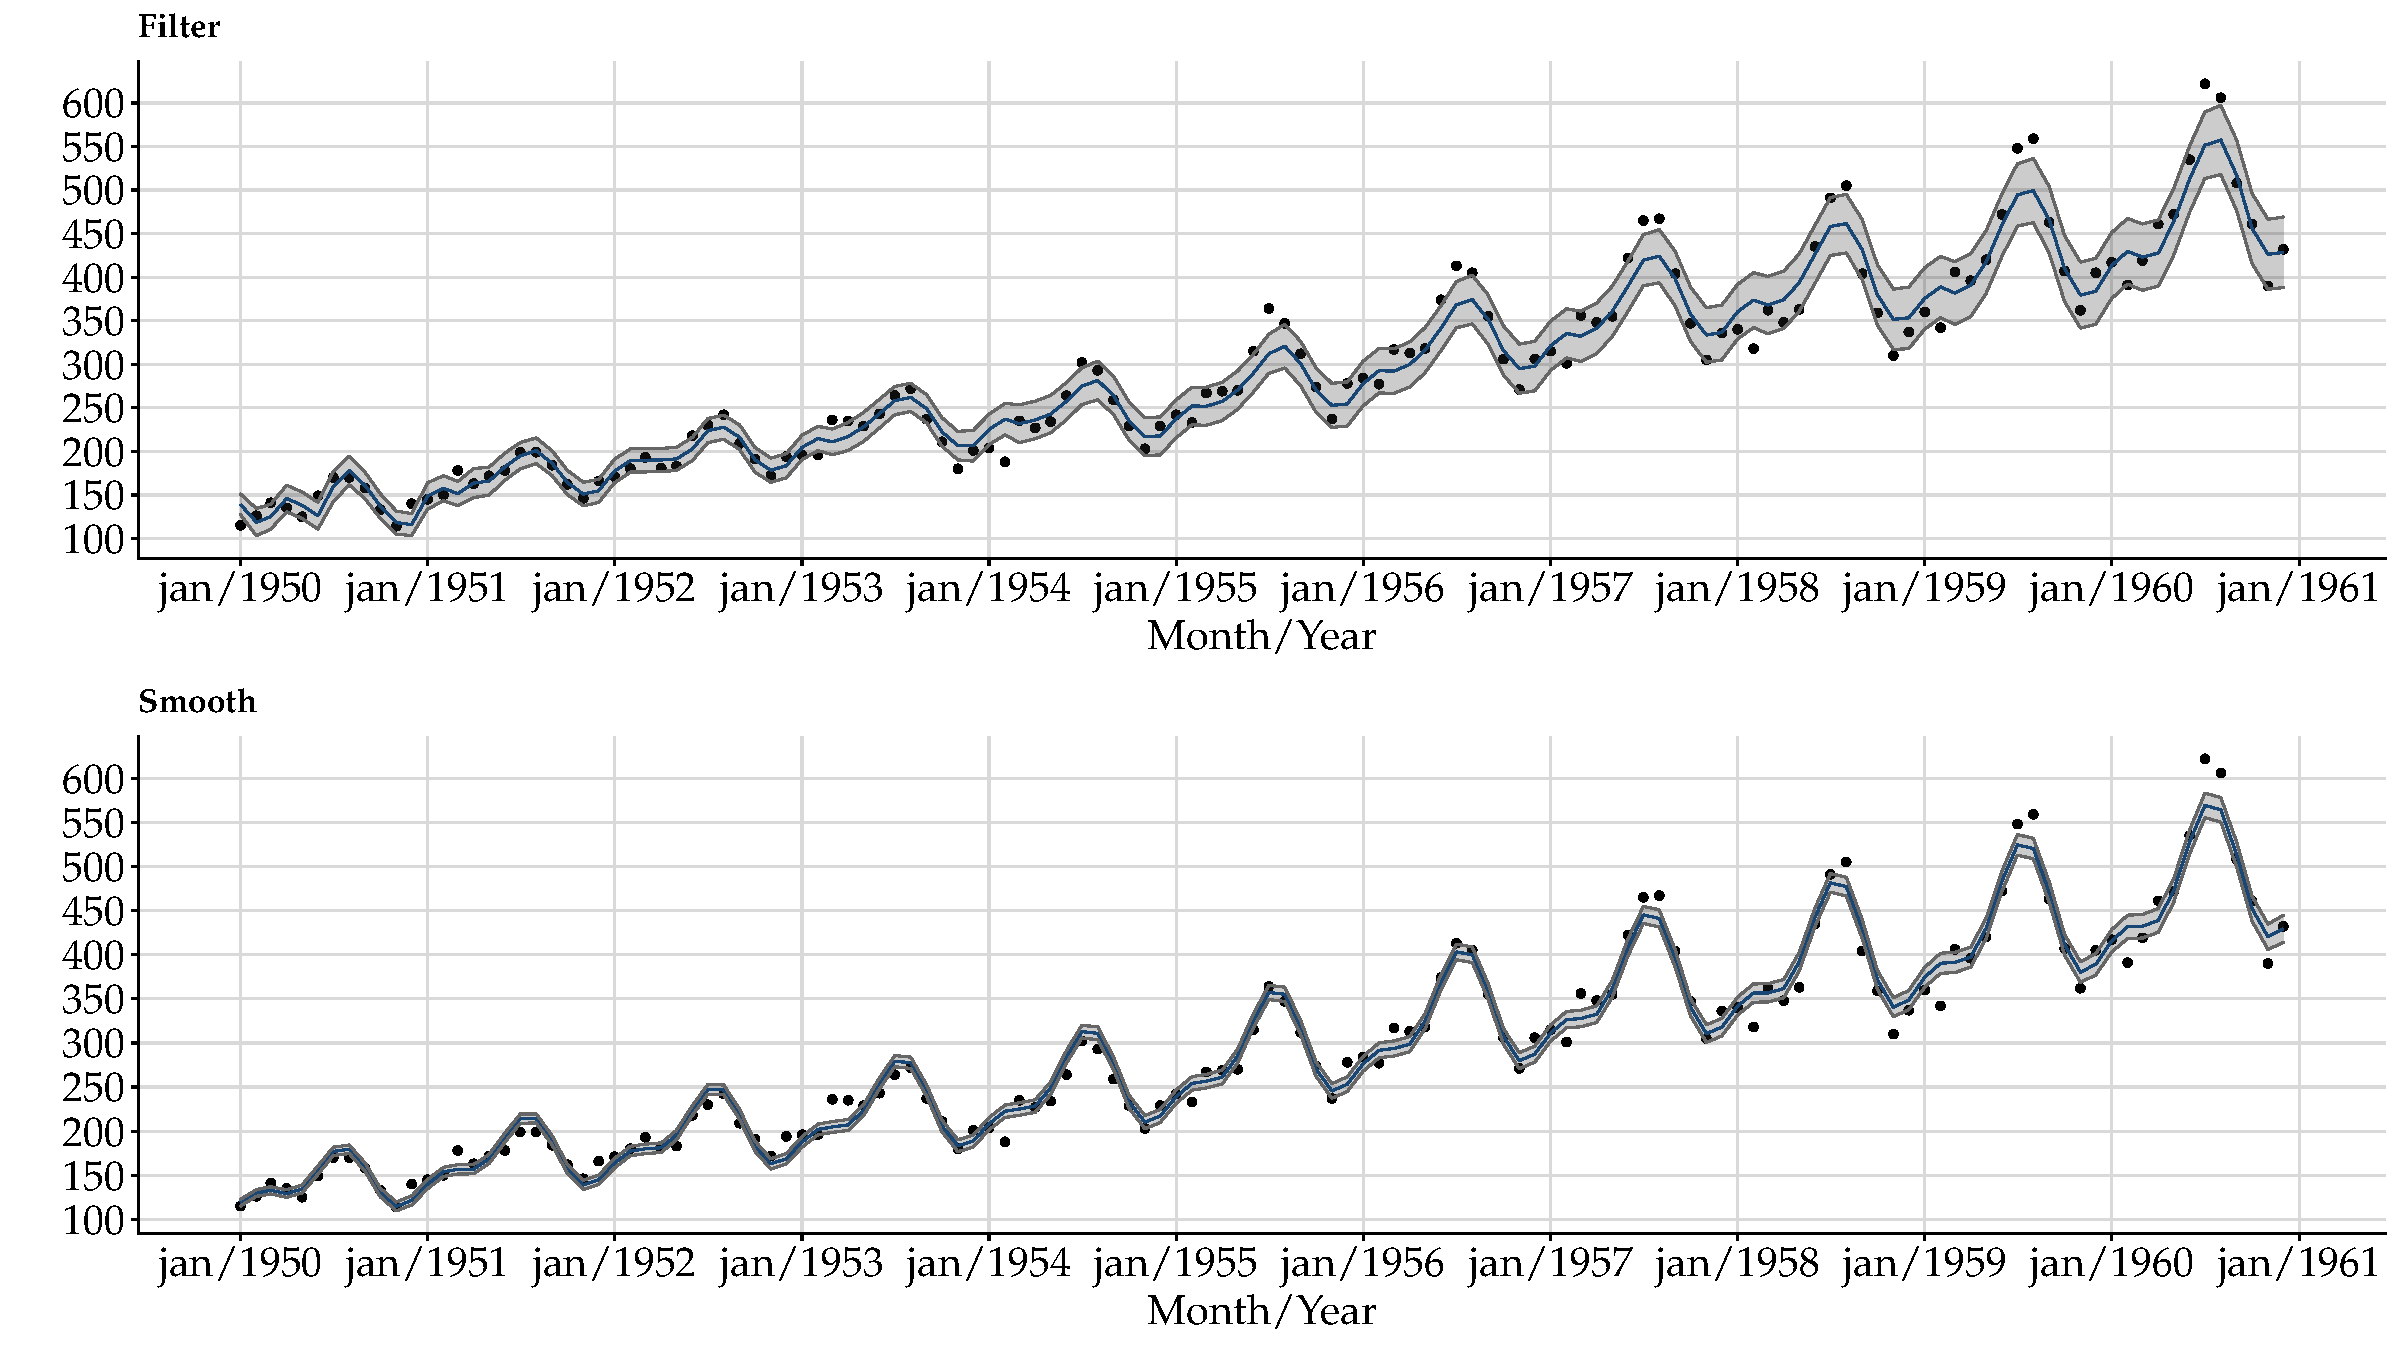
\includegraphics[width=0.9\linewidth]{pybats_detection_files/figure-latex/plots for airpassangers example-1} 

}

\caption{Mean response for Filtered and Smoothed predictive distributions with $95\%$ credible intervals.}\label{fig:plots for airpassangers example}
\end{figure}

Since the seasonality was modeled using harmonic components, the model
has a total of six parameters: level, growth and four for seasonality
(\(a_1, b_1, a_2, b_2\)). For simplicity, the results for de posterior
distributions considered the sum of the harmonic components, whose
moments are given by

\[
\mu_{seas} = \mathbf{F}_{seas}^{\prime} \mathbf{a}_T(-k), \quad \quad \sigma^2_{seas} = \mathbf{F}_{seas}^{\prime} \mathbf{R}_T(-k) \mathbf{F}_{seas}
\] where \(\mathbf{F}_{seas}^{\prime} = [0,0,1,0,1, 0]\). The results
are illustrated below.

\begin{figure}

{\centering 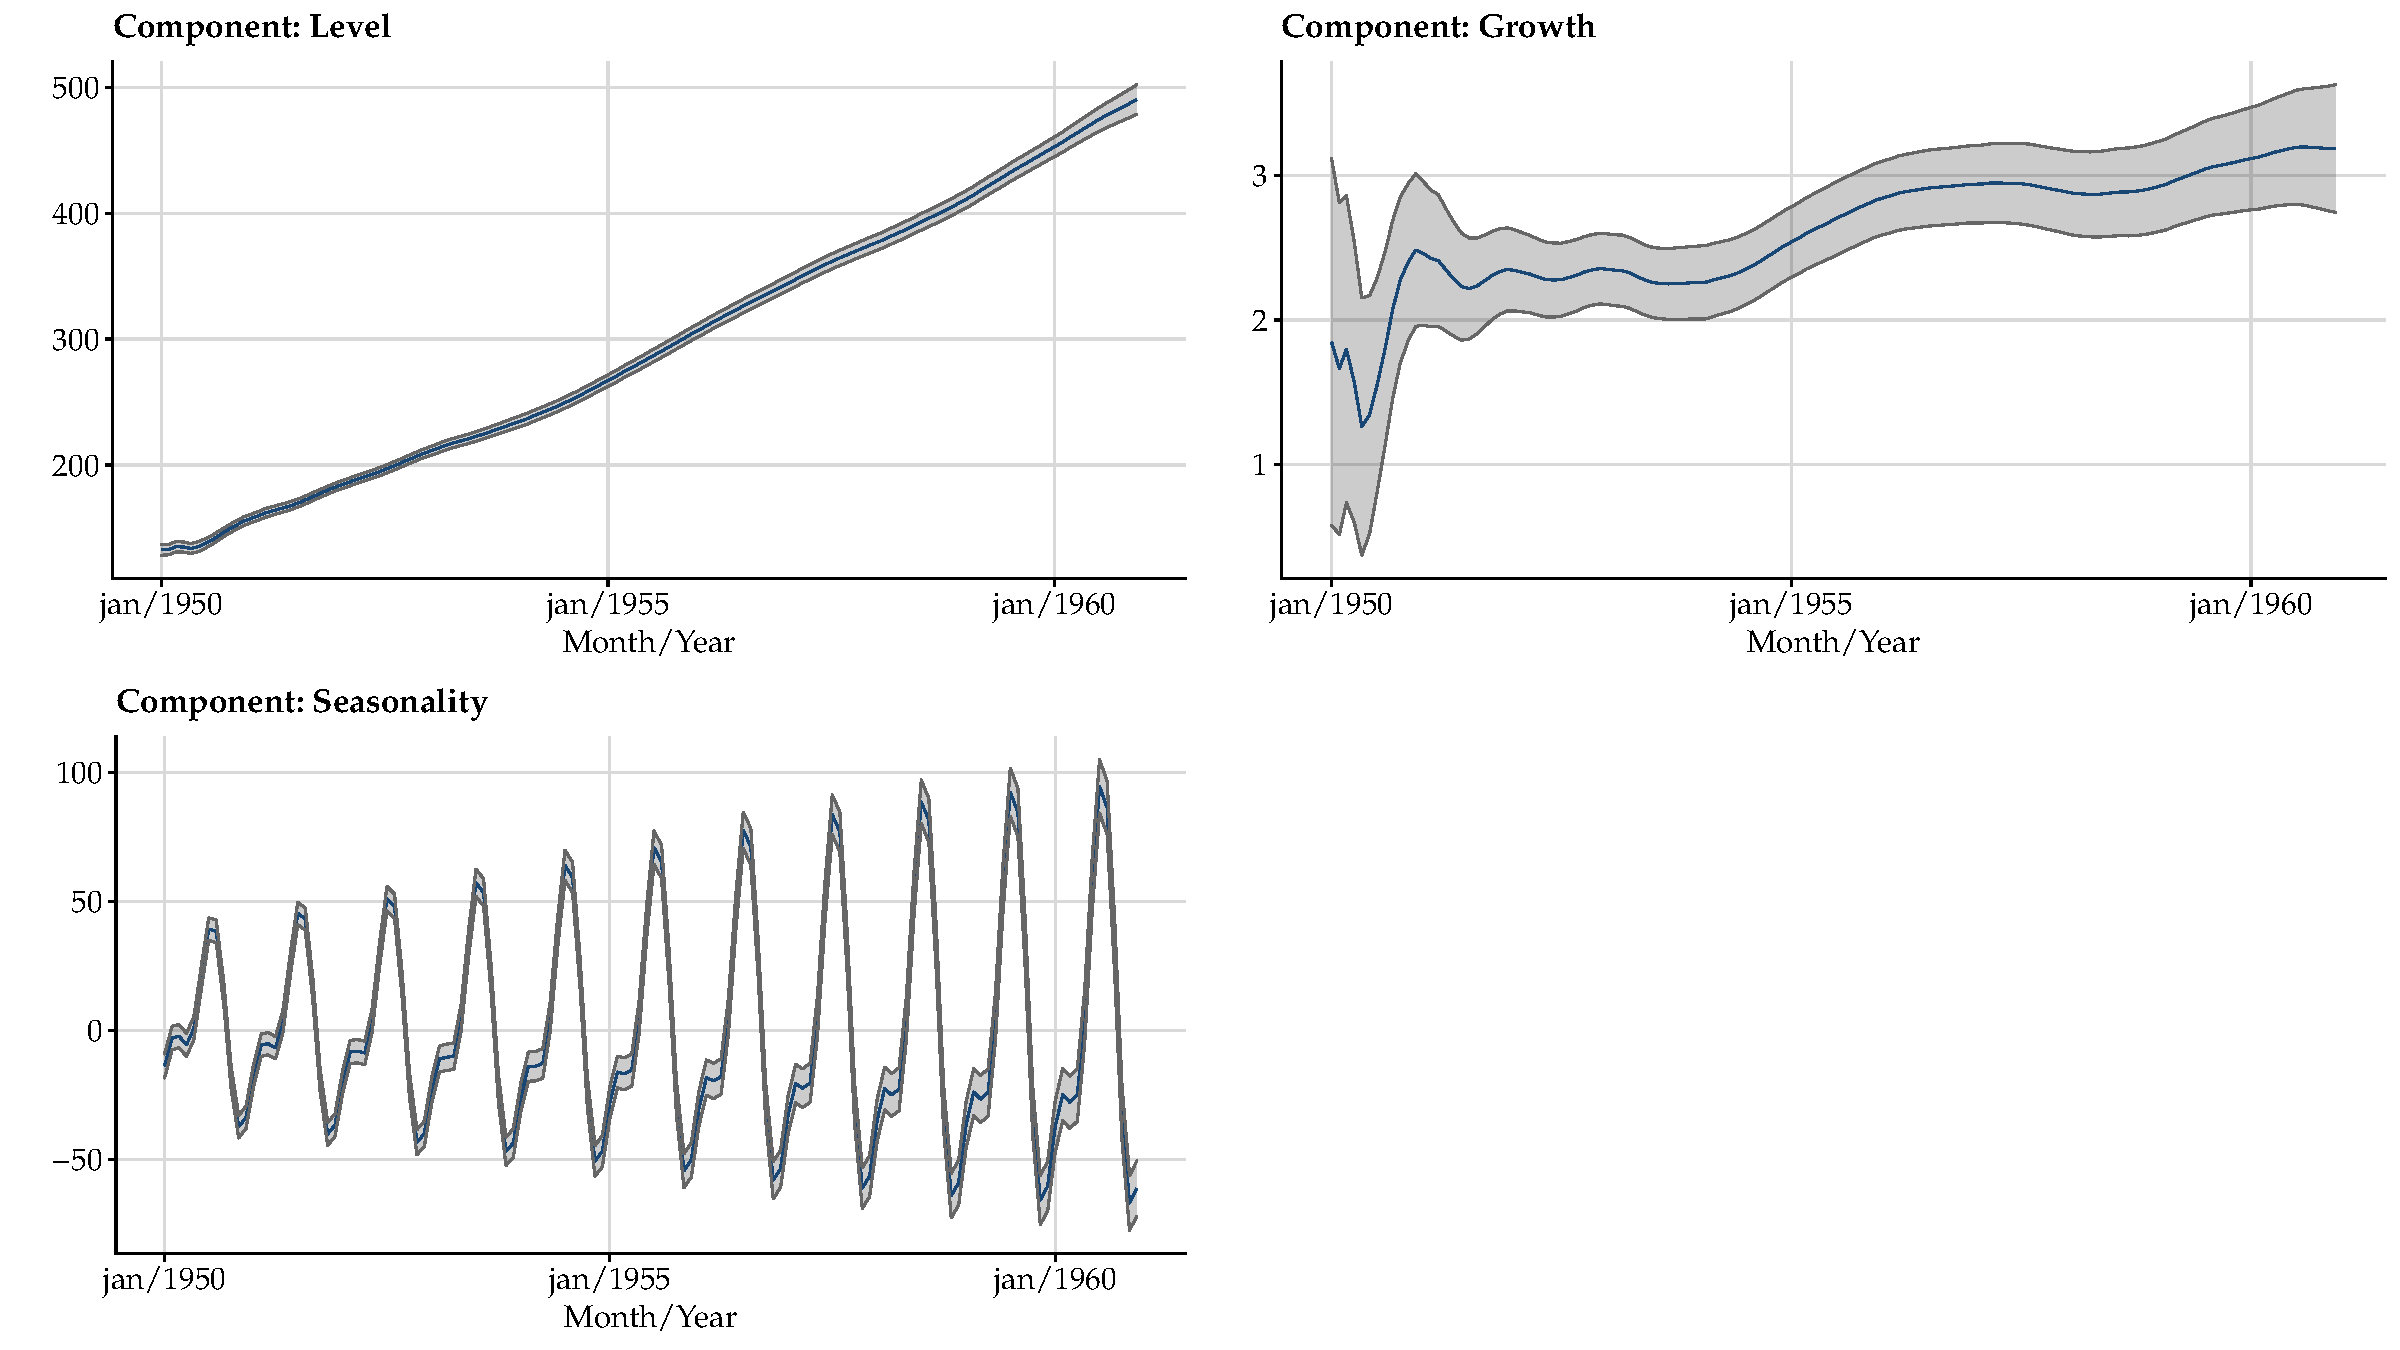
\includegraphics[width=0.9\linewidth]{pybats_detection_files/figure-latex/components for airpassangers example-1} 

}

\caption{Mean response for Filtered and Smoothed posterior distributions for each model component with $95\%$ credible intervals.}\label{fig:components for airpassangers example}
\end{figure}

\hypertarget{manual-intervention}{%
\section{Manual Intervention}\label{manual-intervention}}

\hypertarget{cp6}{%
\subsection{CP6}\label{cp6}}

To illustrate the subjective intervention class we use the CP6 data
graphed below. This time series runs from January 1955 to December 1959,
providing monthly total sales, in monetary terms on a standard scale, of
a product by a major company in UK. Note that the use of standard time
series models may not wield satisfactory results as there a some points
that need some attention:

\begin{enumerate}
\def\labelenumi{\arabic{enumi}.}
\tightlist
\item
  During 1955 the market grows fast at a fast but steady rate,
\item
  A jump in December 1955.
\item
  The sales flattens off for 1956.
\item
  There is a major jump in the sales level in early 1957.
\item
  Another jump in early 1958.
\item
  Throughout the final two years, there is a steady decline back to late
  1957.
\end{enumerate}

\begin{Shaded}
\begin{Highlighting}[]
\OperatorTok{\textgreater{}\textgreater{}\textgreater{}}\NormalTok{ cp6 }\OperatorTok{=}\NormalTok{ load\_cp6()}
\end{Highlighting}
\end{Shaded}

\begin{figure}

{\centering 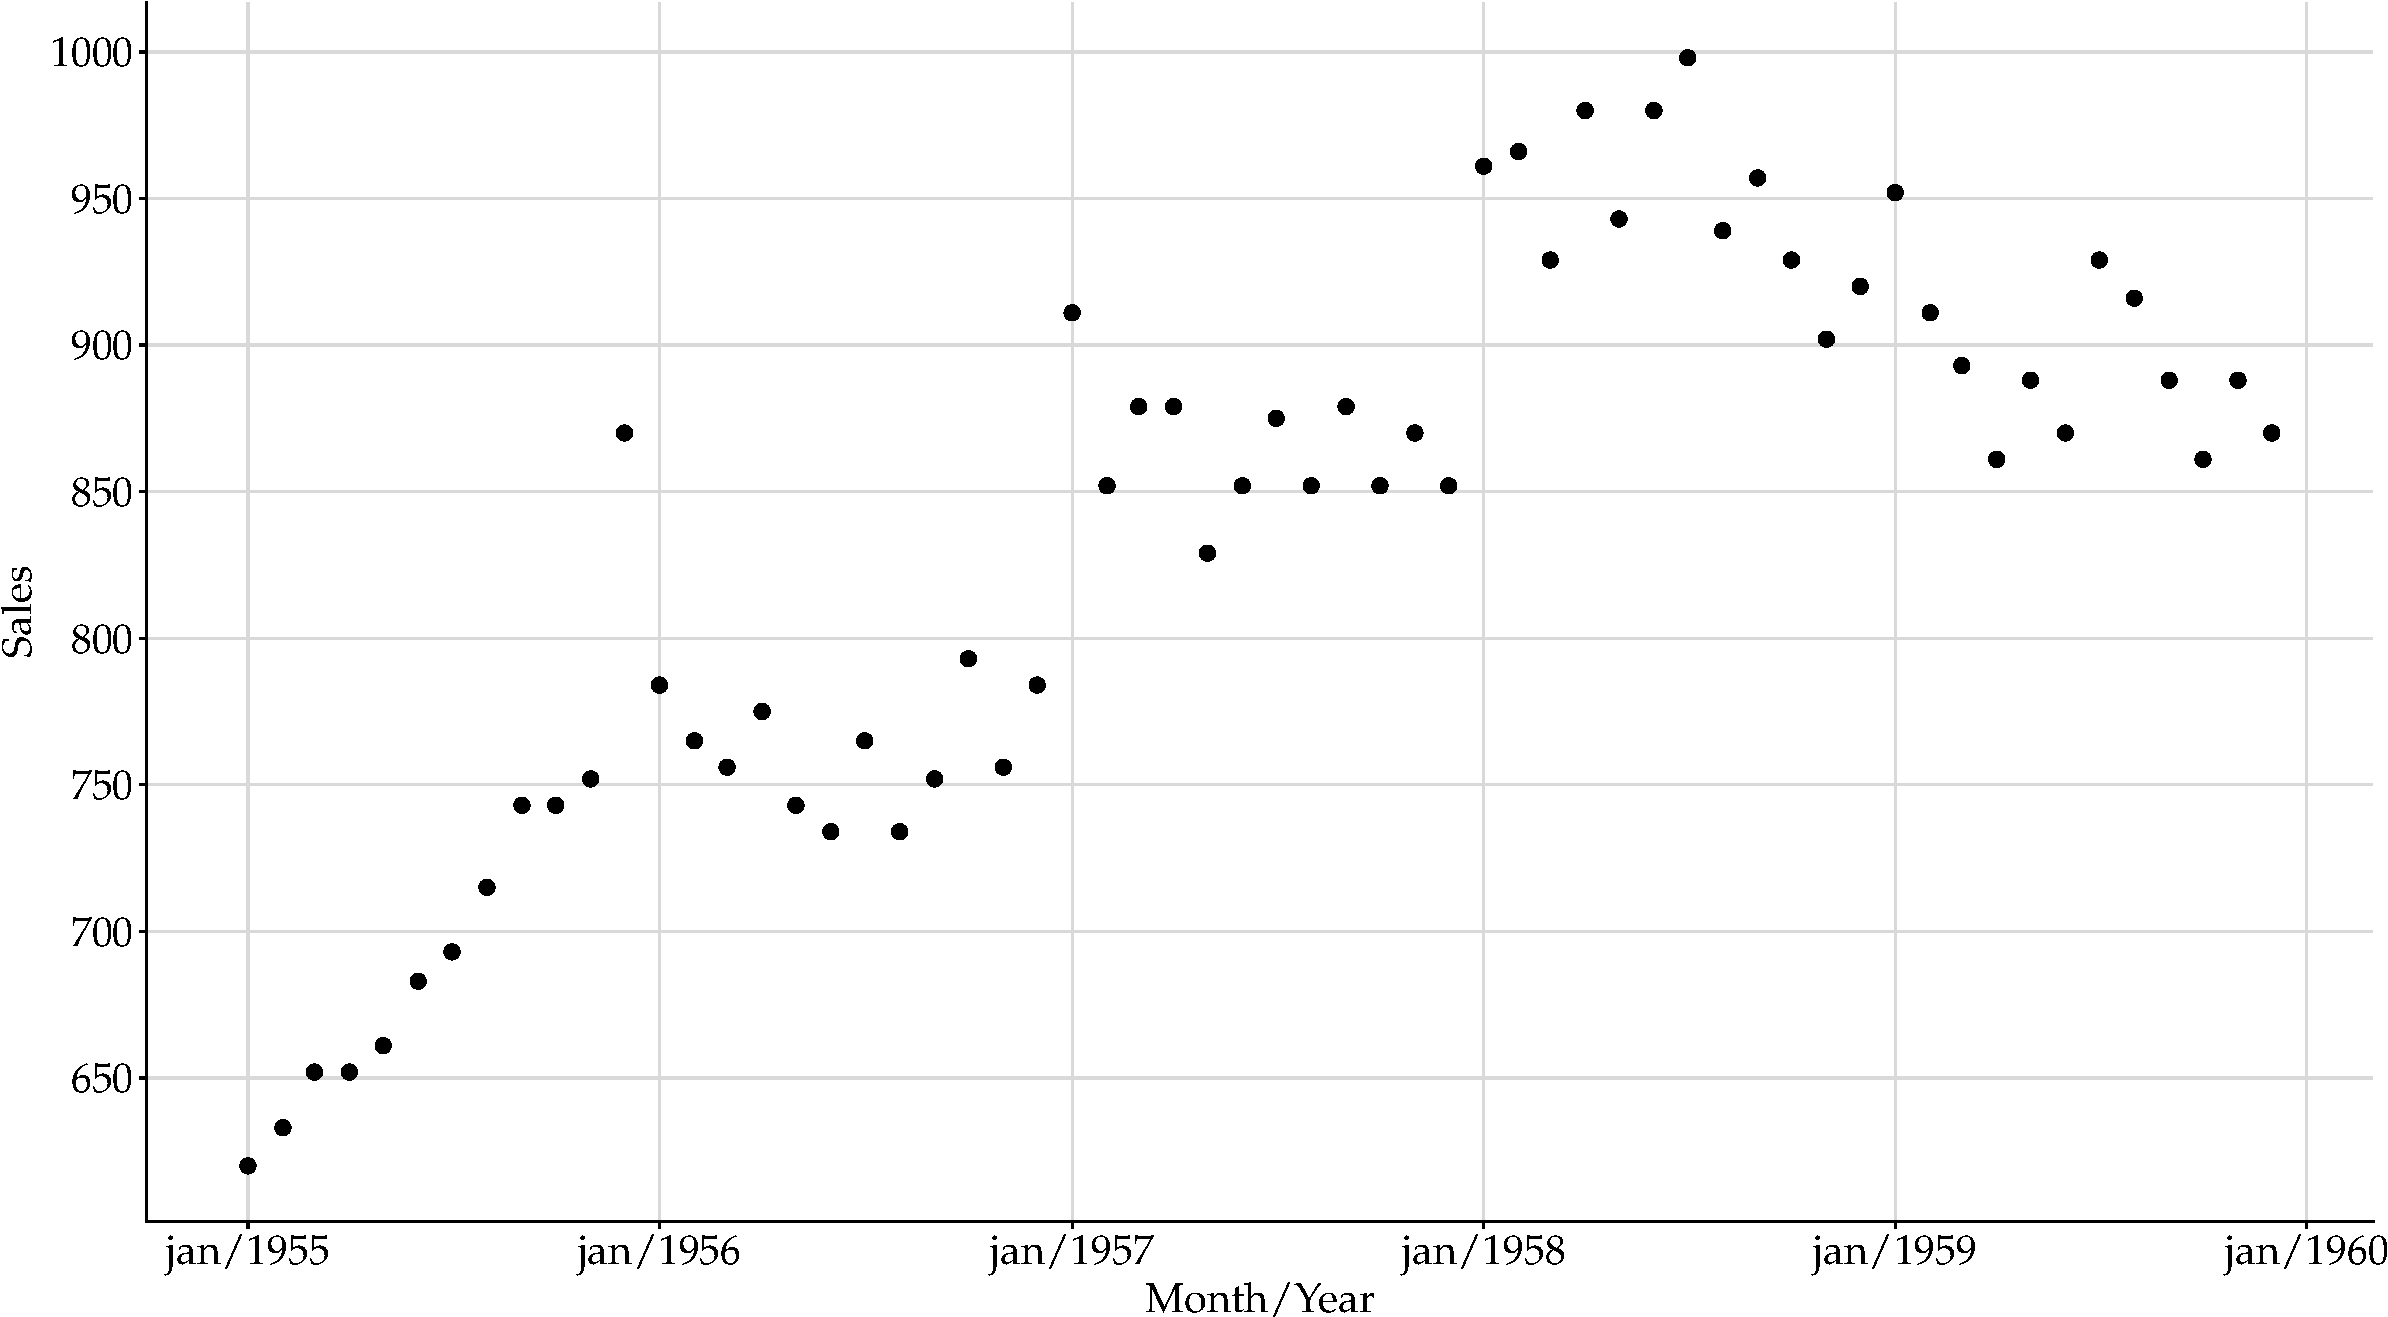
\includegraphics[width=0.9\linewidth]{pybats_detection_files/figure-latex/plot-cp6-1} 

}

\caption{CP6 sales series}\label{fig:plot-cp6}
\end{figure}

\hypertarget{fit-without-intervention}{%
\subsection{Fit Without Intervention}\label{fit-without-intervention}}

Given this, let's see how a standard dlm performs. The model used is
defined below.

\begin{Shaded}
\begin{Highlighting}[]
\OperatorTok{\textgreater{}\textgreater{}\textgreater{}} \CommentTok{\# Define the growth model}
\OperatorTok{\textgreater{}\textgreater{}\textgreater{}}\NormalTok{ a }\OperatorTok{=}\NormalTok{ np.array([}\DecValTok{600}\NormalTok{, }\DecValTok{1}\NormalTok{])}
\OperatorTok{\textgreater{}\textgreater{}\textgreater{}}\NormalTok{ R }\OperatorTok{=}\NormalTok{ np.array([[}\DecValTok{100}\NormalTok{, }\DecValTok{0}\NormalTok{], [}\DecValTok{0}\NormalTok{, }\DecValTok{25}\NormalTok{]])}
\OperatorTok{\textgreater{}\textgreater{}\textgreater{}}\NormalTok{ mod }\OperatorTok{=}\NormalTok{ dlm(a, R, ntrend}\OperatorTok{=}\DecValTok{2}\NormalTok{, deltrend}\OperatorTok{=}\NormalTok{[}\FloatTok{0.90}\NormalTok{, }\FloatTok{0.98}\NormalTok{])}
\end{Highlighting}
\end{Shaded}

\begin{Shaded}
\begin{Highlighting}[]
\OperatorTok{\textgreater{}\textgreater{}\textgreater{}} \CommentTok{\# Filter and Smooth without intervention}
\OperatorTok{\textgreater{}\textgreater{}\textgreater{}}\NormalTok{ smooth }\OperatorTok{=}\NormalTok{ Smoothing(mod}\OperatorTok{=}\NormalTok{mod)}
\OperatorTok{\textgreater{}\textgreater{}\textgreater{}}\NormalTok{ out\_no\_int }\OperatorTok{=}\NormalTok{ smooth.fit(y}\OperatorTok{=}\NormalTok{cp6[}\StringTok{"sales"}\NormalTok{])}
\OperatorTok{\textgreater{}\textgreater{}\textgreater{}}\NormalTok{ dict\_filter\_no\_int }\OperatorTok{=}\NormalTok{ out\_no\_int.get(}\StringTok{"filter"}\NormalTok{).get(}\StringTok{"predictive"}\NormalTok{)}
\end{Highlighting}
\end{Shaded}

\begin{figure}

{\centering 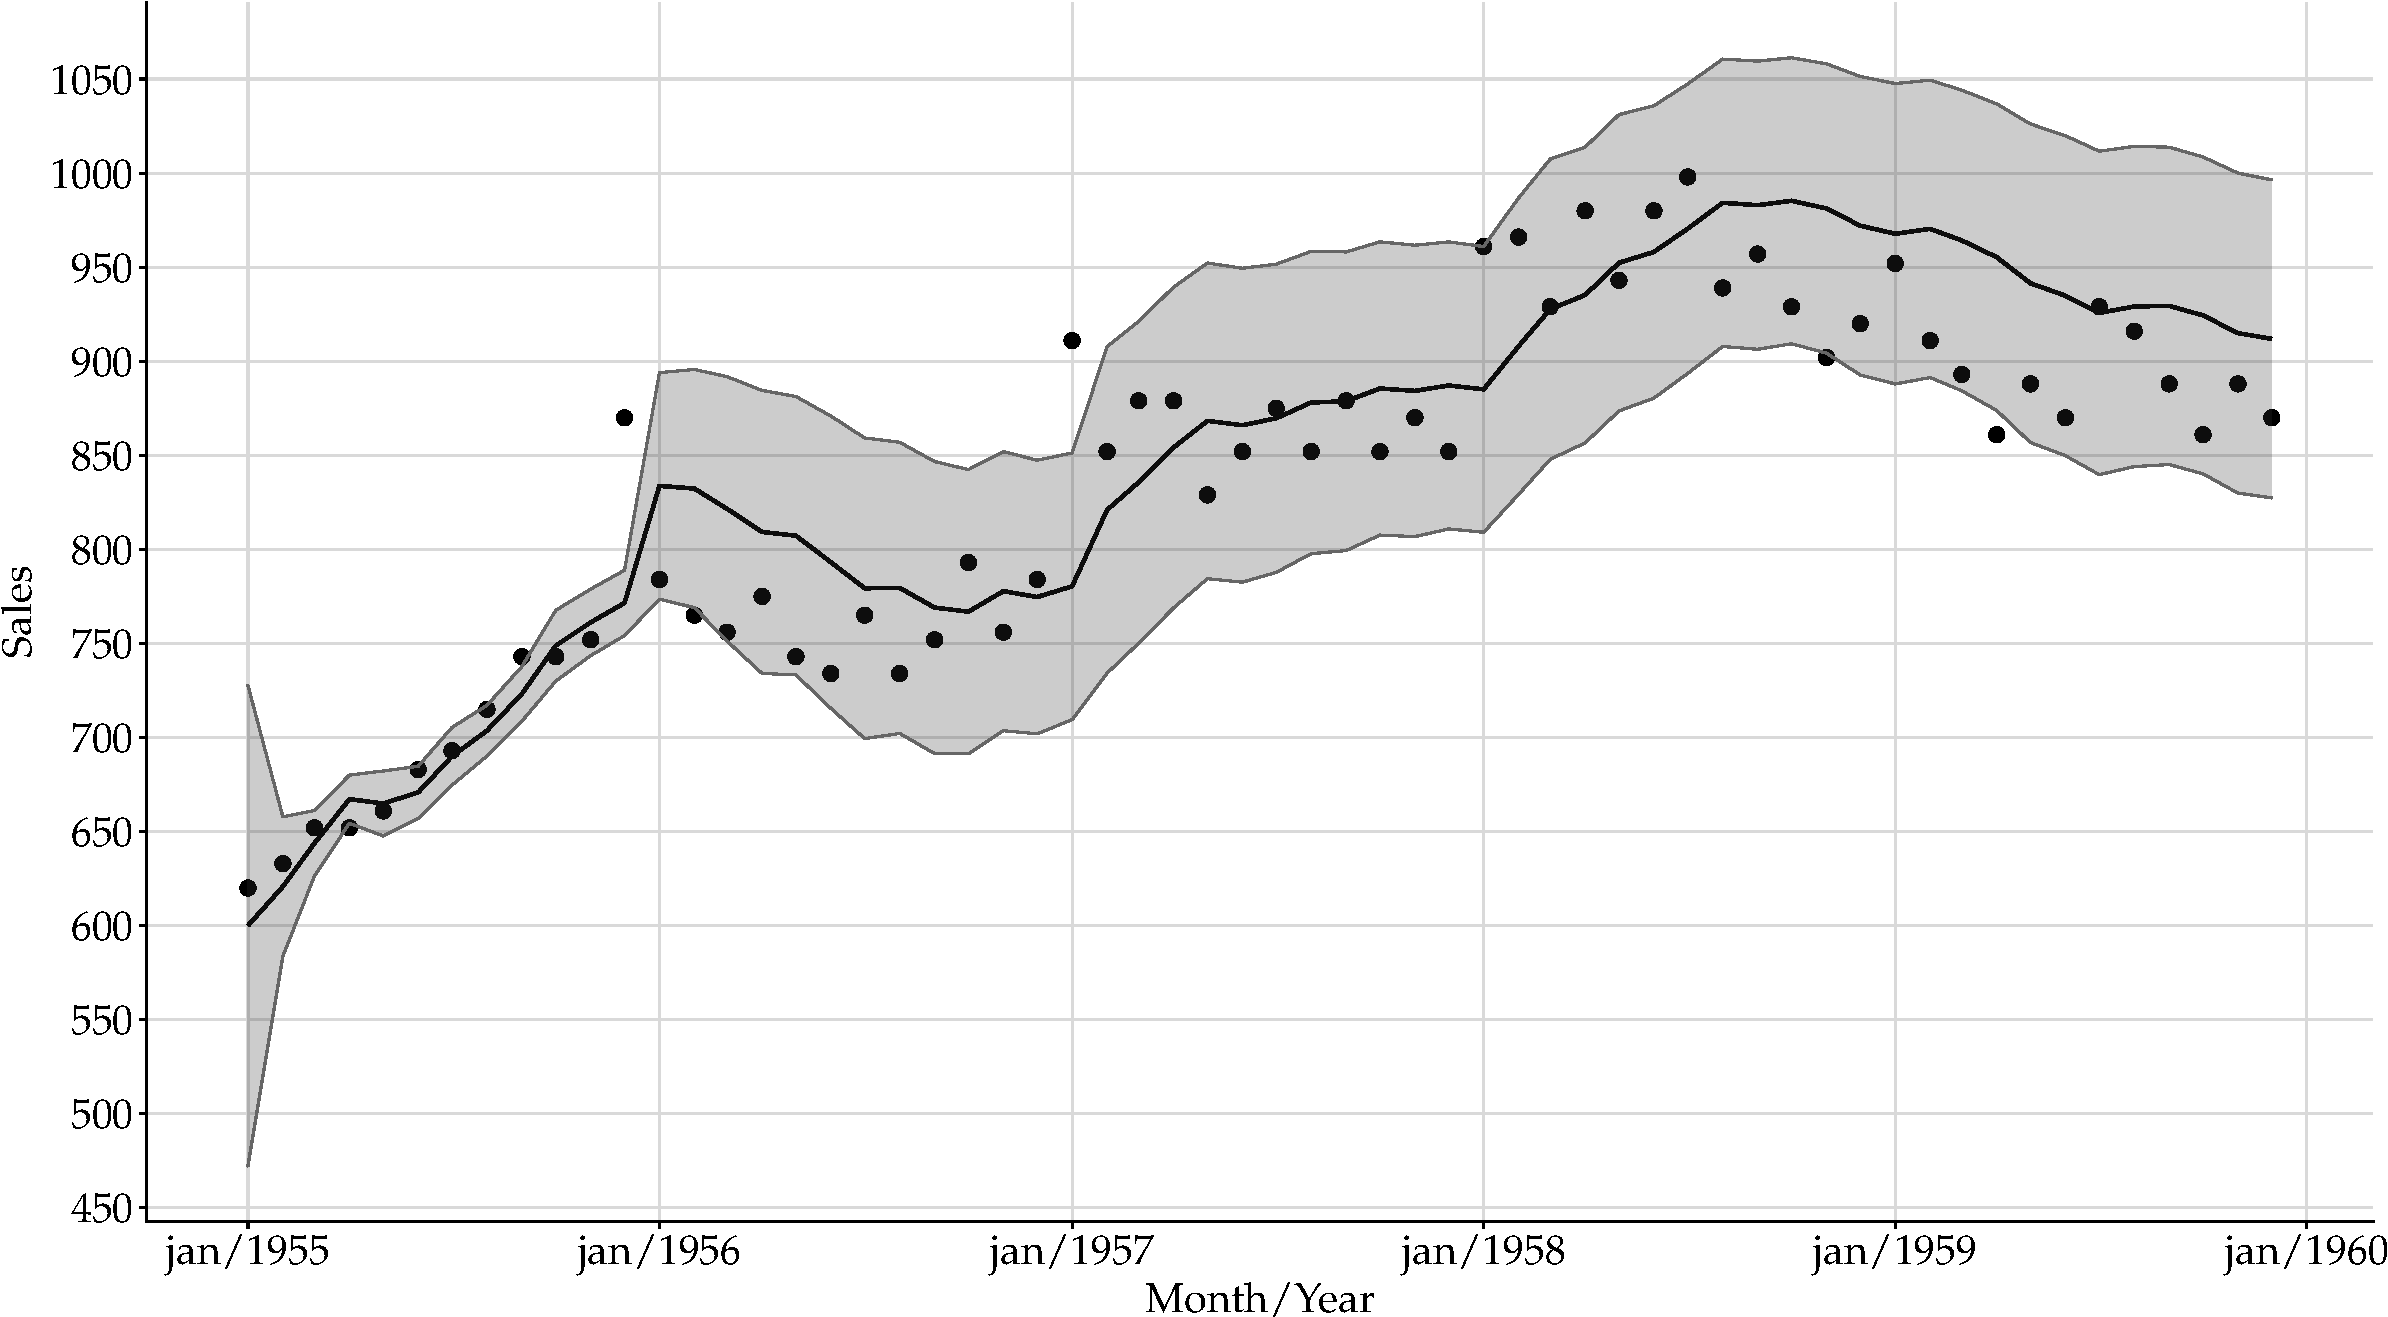
\includegraphics[width=0.9\linewidth]{pybats_detection_files/figure-latex/plot-fit-cp6-filter-no-intervention-1} 

}

\caption{Mean response for Filtered predictive distribution with $95\%$ credible interval}\label{fig:plot-fit-cp6-filter-no-intervention}
\end{figure}

Note that until November 1955 the forecast distribution was quite
acceptable, the credible interval was relatively small and the errors
was were distributed around zero and inside the interval. But with the
jump in December 1955 the level rises dramatically, the biggest problem
is not the model's inability to efficiently predict this point, but the
influence it has on future predictions. Note that for most of the year
1956 the predicted sales overestimation the real sales, giving a cluster
of negative errors \((y_t - f_t)\). In early 1957 another jump was
observed, but in this case, it was accompanied by a regime change. And
this has great impact in the amplitude of the credible intervals. In
early 1958 another regime change, followed by a change in grow, that is
not properly modeled since from August 1958 to January 1960 all errors
were negative with the exception of July 1959.

\hypertarget{fit-with-intervention}{%
\subsection{Fit With Intervention}\label{fit-with-intervention}}

With the intervention class it is possible to consider outside
information to define the prior distribution at the time \(t\). This can
be done in two ways: noise or subjective. Which must be provided in a
list of dictionaries containing the time the intervention will be
carried out and the type. Lets start with a empty list

\begin{Shaded}
\begin{Highlighting}[]
\OperatorTok{\textgreater{}\textgreater{}\textgreater{}}\NormalTok{ intervention\_list }\OperatorTok{=}\NormalTok{ []}
\end{Highlighting}
\end{Shaded}

\hypertarget{noise-intervention-in-prior-variance}{%
\subsubsection{Noise Intervention in Prior
Variance}\label{noise-intervention-in-prior-variance}}

In our example, suppose that a change in growth for the year 1956 was
anticipated. An increase in uncertainty about level and growth can be
done by the addition of a matrix \(H_t\) to \(R_t\) at time \(t=12\)
given by

\[
  H_t = \begin{bmatrix}
    100 & 25 \\
    25 & 25
  \end{bmatrix}
\] Thus, there is an increase (a positive shift) in the prior variance
of the components. In our list of interventions we have

\begin{Shaded}
\begin{Highlighting}[]
\OperatorTok{\textgreater{}\textgreater{}\textgreater{}}\NormalTok{ intervention\_list }\OperatorTok{=}\NormalTok{ [\{}
\OperatorTok{\textgreater{}\textgreater{}\textgreater{}}   \StringTok{"time\_index"}\NormalTok{: }\DecValTok{12}\NormalTok{, }\StringTok{"which"}\NormalTok{: [}\StringTok{"noise"}\NormalTok{],}
\OperatorTok{\textgreater{}\textgreater{}\textgreater{}}   \StringTok{"parameters"}\NormalTok{: [\{}
\OperatorTok{\textgreater{}\textgreater{}\textgreater{}}     \StringTok{"h\_shift"}\NormalTok{: np.array([}\DecValTok{0}\NormalTok{, }\DecValTok{0}\NormalTok{]),}
\OperatorTok{\textgreater{}\textgreater{}\textgreater{}}     \StringTok{"H\_shift"}\NormalTok{: np.array([[}\DecValTok{100}\NormalTok{, }\DecValTok{25}\NormalTok{], [}\DecValTok{25}\NormalTok{, }\DecValTok{25}\NormalTok{]])\}]}
\OperatorTok{\textgreater{}\textgreater{}\textgreater{}}\NormalTok{ \}]}
\end{Highlighting}
\end{Shaded}

where

\begin{itemize}
\tightlist
\item
  \texttt{time\_index}: time of intervention;
\item
  \texttt{which}: type of intervention (in this case, a noise
  intervention);
\item
  \texttt{parameters}: the values for the intervention.

  \begin{itemize}
  \tightlist
  \item
    \texttt{h\_shit}: Shift in mean (we'll see more about that later).
  \item
    \texttt{H\_shift}: Shift in variance.
  \end{itemize}
\end{itemize}

\hypertarget{noise-intervention-in-prior-mean-and-variance}{%
\subsubsection{Noise Intervention in Prior Mean and
Variance}\label{noise-intervention-in-prior-mean-and-variance}}

It is also possible to intervene in the prior mean. Suppose an increase
in the market level is expected for the year 1957, we can add a change
in level of 80 units and increase the variance by 100 at January
\((t=25)\)

\[
\mathbf{h}_{25} = \begin{bmatrix}
80 \\ 
0
\end{bmatrix} 
\quad 
\text{and}
\quad 
\mathbf{H}_{25} = \begin{bmatrix}
100 & 0 \\
0 & 0
\end{bmatrix}
\]

now, updating our intervention list

\begin{Shaded}
\begin{Highlighting}[]
\OperatorTok{\textgreater{}\textgreater{}\textgreater{}}\NormalTok{ intervention\_list }\OperatorTok{=}\NormalTok{ [\{}
\OperatorTok{\textgreater{}\textgreater{}\textgreater{}}   \StringTok{"time\_index"}\NormalTok{: }\DecValTok{12}\NormalTok{, }\StringTok{"which"}\NormalTok{: [}\StringTok{"noise"}\NormalTok{],}
\OperatorTok{\textgreater{}\textgreater{}\textgreater{}}   \StringTok{"parameters"}\NormalTok{: [\{}
\OperatorTok{\textgreater{}\textgreater{}\textgreater{}}     \StringTok{"h\_shift"}\NormalTok{: np.array([}\DecValTok{0}\NormalTok{, }\DecValTok{0}\NormalTok{]),}
\OperatorTok{\textgreater{}\textgreater{}\textgreater{}}     \StringTok{"H\_shift"}\NormalTok{: np.array([[}\DecValTok{100}\NormalTok{, }\DecValTok{25}\NormalTok{], [}\DecValTok{25}\NormalTok{, }\DecValTok{25}\NormalTok{]])\}], }
\OperatorTok{\textgreater{}\textgreater{}\textgreater{}}     
\OperatorTok{\textgreater{}\textgreater{}\textgreater{}}   \StringTok{"time\_index"}\NormalTok{: }\DecValTok{25}\NormalTok{, }\StringTok{"which"}\NormalTok{: [}\StringTok{"noise"}\NormalTok{],}
\OperatorTok{\textgreater{}\textgreater{}\textgreater{}}   \StringTok{"parameters"}\NormalTok{: [\{}
\OperatorTok{\textgreater{}\textgreater{}\textgreater{}}     \StringTok{"h\_shift"}\NormalTok{: np.array([}\DecValTok{80}\NormalTok{, }\DecValTok{0}\NormalTok{]),}
\OperatorTok{\textgreater{}\textgreater{}\textgreater{}}     \StringTok{"H\_shift"}\NormalTok{: np.array([[}\DecValTok{100}\NormalTok{, }\DecValTok{0}\NormalTok{], [}\DecValTok{0}\NormalTok{, }\DecValTok{0}\NormalTok{]])\}]}
\OperatorTok{\textgreater{}\textgreater{}\textgreater{}}\NormalTok{ \}]}
\end{Highlighting}
\end{Shaded}

In January 1958 \((t=37)\) another jump in level is anticipated, this
time of about 100 units with a feeling of increased certainly about the
new level and also a anticipated uncertainly for the growth. At this
time, the prior mean and variance given by

\[
\mathbf{a}_{37} = \begin{bmatrix}
864.5 \\
0
\end{bmatrix}
\quad 
\text{and}
\quad 
\mathbf{R}_{37} = \begin{bmatrix}
91.7 & 9.2 \\
9.2 & 1.56
\end{bmatrix}
\]

are simply altered to

\[
\mathbf{a}^{*}_{37} = \begin{bmatrix}
970 \\
0
\end{bmatrix}
\quad 
\text{and}
\quad 
\mathbf{R}^{*}_{37} = \begin{bmatrix}
50 & 0 \\
0 & 5
\end{bmatrix}
\]

\hypertarget{observational-variance-intervention}{%
\subsubsection{Observational Variance
Intervention}\label{observational-variance-intervention}}

It is also possible to perform interventions on observational variance.
This can be useful for outlier anticipation.

Suppose that at the end of 1955 there will be an announcement of future
price increases which will result in forward-buying. So, a intervention
at December 1955 \((t=12)\) will allow for an anticipated outlier. In
late 1956, there is a a view that the marked change in the new year will
begin with a maverick value, as the product that are to be discontinued
are sold cheaply.

This interventions can be done by including a variance intervention in
our list of interventions for the respective time:

\begin{Shaded}
\begin{Highlighting}[]
\OperatorTok{\textgreater{}\textgreater{}\textgreater{}}\NormalTok{ list\_interventions }\OperatorTok{=}\NormalTok{ [}
\OperatorTok{\textgreater{}\textgreater{}\textgreater{}}\NormalTok{     \{}\StringTok{"time\_index"}\NormalTok{: }\DecValTok{12}\NormalTok{, }\StringTok{"which"}\NormalTok{: [}\StringTok{"variance"}\NormalTok{, }\StringTok{"noise"}\NormalTok{],}
\OperatorTok{\textgreater{}\textgreater{}\textgreater{}}      \StringTok{"parameters"}\NormalTok{: [\{}\StringTok{"v\_shift"}\NormalTok{: }\StringTok{"ignore"}\NormalTok{\},}
\OperatorTok{\textgreater{}\textgreater{}\textgreater{}}\NormalTok{                     \{}\StringTok{"h\_shift"}\NormalTok{: np.array([}\DecValTok{0}\NormalTok{, }\DecValTok{0}\NormalTok{]),}
\OperatorTok{\textgreater{}\textgreater{}\textgreater{}}                      \StringTok{"H\_shift"}\NormalTok{: np.array([[}\DecValTok{1000}\NormalTok{, }\DecValTok{25}\NormalTok{], [}\DecValTok{25}\NormalTok{, }\DecValTok{25}\NormalTok{]])\}]}
\OperatorTok{\textgreater{}\textgreater{}\textgreater{}}\NormalTok{      \},}
\OperatorTok{\textgreater{}\textgreater{}\textgreater{}}\NormalTok{     \{}\StringTok{"time\_index"}\NormalTok{: }\DecValTok{25}\NormalTok{, }\StringTok{"which"}\NormalTok{: [}\StringTok{"noise"}\NormalTok{, }\StringTok{"variance"}\NormalTok{],}
\OperatorTok{\textgreater{}\textgreater{}\textgreater{}}      \StringTok{"parameters"}\NormalTok{: [\{}\StringTok{"h\_shift"}\NormalTok{: np.array([}\DecValTok{80}\NormalTok{, }\DecValTok{0}\NormalTok{]),}
\OperatorTok{\textgreater{}\textgreater{}\textgreater{}}                      \StringTok{"H\_shift"}\NormalTok{: np.array([[}\DecValTok{100}\NormalTok{, }\DecValTok{0}\NormalTok{], [}\DecValTok{0}\NormalTok{, }\DecValTok{0}\NormalTok{]])\},}
\OperatorTok{\textgreater{}\textgreater{}\textgreater{}}\NormalTok{                     \{}\StringTok{"v\_shift"}\NormalTok{: }\StringTok{"ignore"}\NormalTok{\}]\},}
\OperatorTok{\textgreater{}\textgreater{}\textgreater{}}\NormalTok{     \{}\StringTok{"time\_index"}\NormalTok{: }\DecValTok{37}\NormalTok{, }\StringTok{"which"}\NormalTok{: [}\StringTok{"subjective"}\NormalTok{],}
\OperatorTok{\textgreater{}\textgreater{}\textgreater{}}      \StringTok{"parameters"}\NormalTok{: [\{}\StringTok{"a\_star"}\NormalTok{: np.array([}\DecValTok{970}\NormalTok{, }\DecValTok{0}\NormalTok{]),}
\OperatorTok{\textgreater{}\textgreater{}\textgreater{}}                      \StringTok{"R\_star"}\NormalTok{: np.array([[}\DecValTok{50}\NormalTok{, }\DecValTok{0}\NormalTok{], [}\DecValTok{0}\NormalTok{, }\DecValTok{5}\NormalTok{]])\}]\}}
\OperatorTok{\textgreater{}\textgreater{}\textgreater{}}\NormalTok{ ]}
\end{Highlighting}
\end{Shaded}

\hypertarget{performing-the-fit-filter-and-smoothing-with-interventions}{%
\subsubsection{Performing the fit (filter and smoothing) with
interventions}\label{performing-the-fit-filter-and-smoothing-with-interventions}}

Finally, the fit with intervention can be done using the
\texttt{Intervention} class. In the \texttt{.fit} method we will
initialize the model and the loop forecast, observe and update, this
time with the interventions given in \texttt{list\_interventions},
begin. This will return a dictionary with the same structure as
presented in the smoothing section.

\begin{Shaded}
\begin{Highlighting}[]
\OperatorTok{\textgreater{}\textgreater{}\textgreater{}}\NormalTok{ manual\_interventions }\OperatorTok{=}\NormalTok{ Intervention(mod}\OperatorTok{=}\NormalTok{mod)}
\OperatorTok{\textgreater{}\textgreater{}\textgreater{}}\NormalTok{ out\_int }\OperatorTok{=}\NormalTok{ manual\_interventions.fit(}
\OperatorTok{\textgreater{}\textgreater{}\textgreater{}}\NormalTok{     y}\OperatorTok{=}\NormalTok{cp6[}\StringTok{"sales"}\NormalTok{], interventions}\OperatorTok{=}\NormalTok{list\_interventions)}
\OperatorTok{\textgreater{}\textgreater{}\textgreater{}}\NormalTok{ dict\_filter\_int }\OperatorTok{=}\NormalTok{ out\_int.get(}\StringTok{"filter"}\NormalTok{).get(}\StringTok{"predictive"}\NormalTok{)}
\end{Highlighting}
\end{Shaded}

\begin{figure}

{\centering 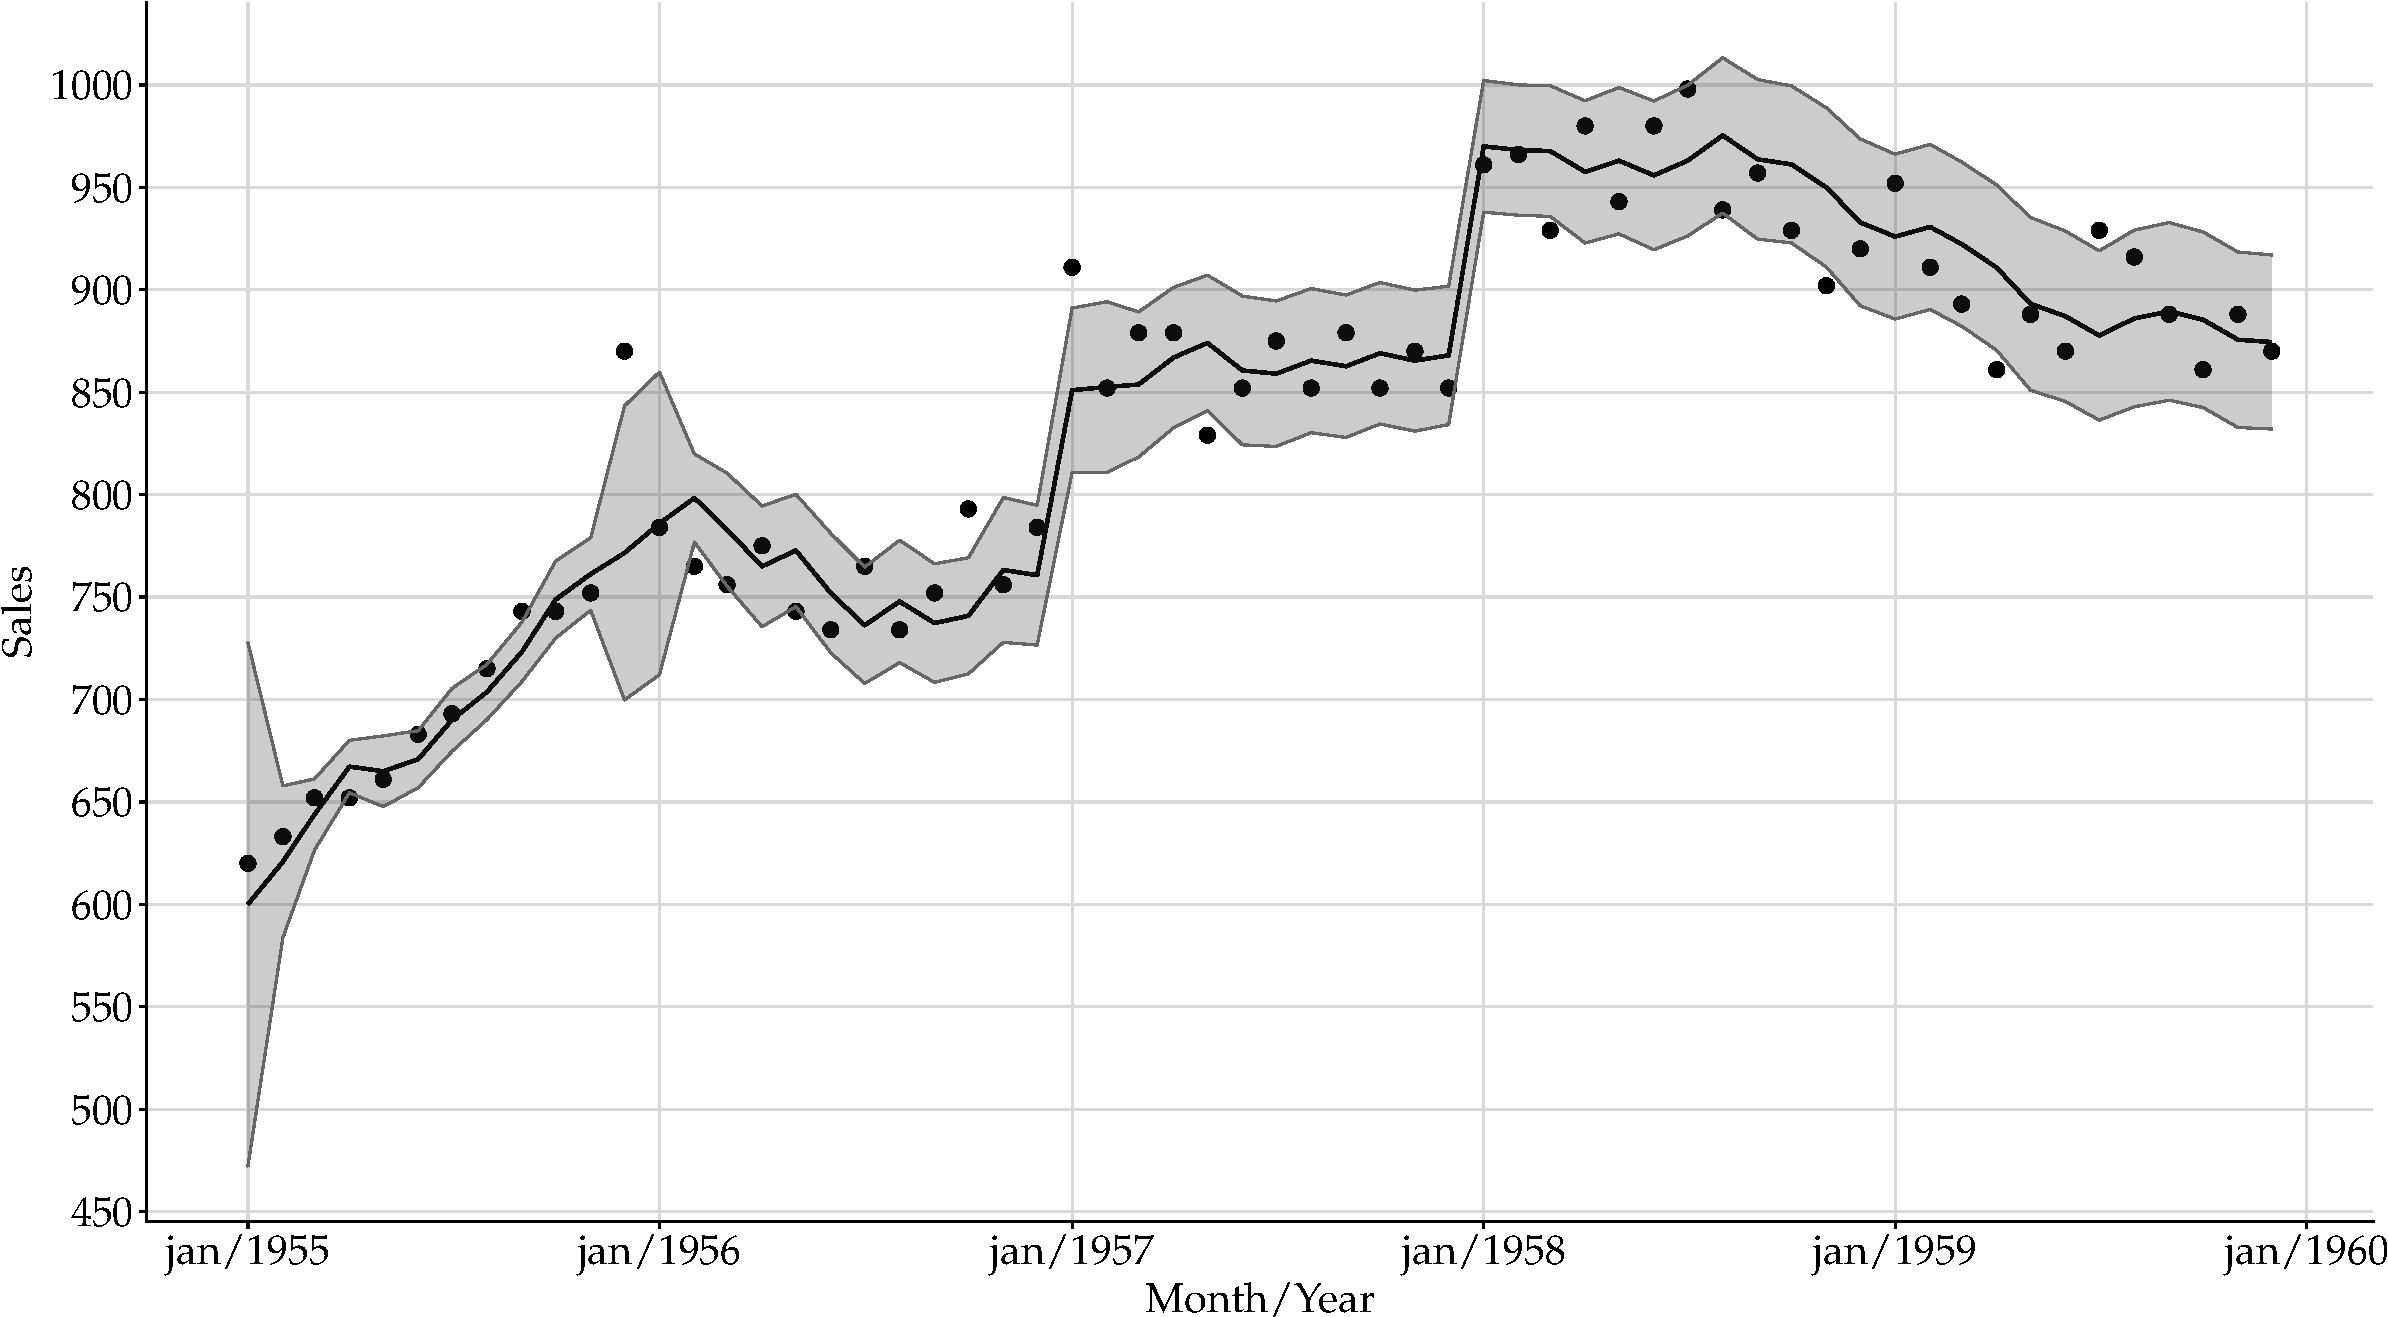
\includegraphics[width=0.9\linewidth]{pybats_detection_files/figure-latex/plot-fit-cp6-filter-intervention-1} 

}

\caption{Mean response for filtered predictive distribution with $95\%$ credible interval and ideal interventions}\label{fig:plot-fit-cp6-filter-intervention}
\end{figure}

\hypertarget{automatic-monitoring}{%
\section{Automatic Monitoring}\label{automatic-monitoring}}

The automatic monitoring method sequentially evaluate the forecasting
activity to detect breakdowns, based on Bayes factor for two models
\(M_0\) versus \(M_1\) with same mathematical structure, differing only
through the values for \(\boldsymbol{\theta}_t\) or simply the discount
factors. Let \(M_0\) be a standard DLM without intervention and \(M_1\)
and alternative model that is introduced to provide assessment of
\(M_0\) by comparison. The Bayes' factor for the observed value \(y_t\)
is given by

\[
H_t = p_0(y_t \vert D_{t-1}) / p_1(y_t \vert D_{t-1}),
\] where \(p_0\) and \(p_1\) are the predictive densities at time \(t\)
for \(M_0\) and \(M_1\).If \(H_t\) is small then the \(M_1\) model is
preferred. For \(k=1, \dots, t\) last consecutive observations
\(y_t, y_{t-1}, y_{t-k+1}\) the local Bayes factor is given by \[
H_t(k) = \prod_{r=t-k+1}^t H_r = \frac{p_0 (y_t, y_{t-1}, \dots, y_{t-k+1})}{p_1 (y_t, y_{t-1}, \dots, y_{t-k+1})}.
\] and the cumulative Bayes factor \((L_t)\) is \[
L_t = \min_{1\leq k \leq t} H_t(k), \\
\] the minimum at time \(t\) is taken at \(k=l_t\), with
\(L_t = H_t(l_t)\) and \(l_t\) being a integer given by \[
l_t = (1+l_{t-1}) I(L_{t-1} < 1) + I(L_{t-1} \geq 1),
\] where \(I(\cdot)\) is a indicator function.

Basically, \(H_t\) is initially used to indicate if \(y_t\) is a outlier
when \(H_t < \tau\) (which represent preference for \(M_1\)). However a
small Bayes factor may indicate the start of a regime change, in this
case we need to accumulate evidences. For this \(L_t\) and \(l_t\) are
used. The automatic detection is done following the steps

\begin{itemize}
\tightlist
\item
  If \(H_t \leq \tau\), then \(y_t\) is a outlier and is omitted from
  the analysis.
\item
  If \(H_t > \tau\), we must look at \(L_t\) for cumulative evidence
  against \(M_0\).

  \begin{itemize}
  \tightlist
  \item
    If \(L_t < \tau\) or \(l_t > 2\) then a parametric chance is
    detected \(M_1\) is adopted.
  \end{itemize}
\end{itemize}

It is also possible to consider two alternative models \(M_1\) and
\(M_2\), this is useful for identification of outliers/regime change in
two directions.

\hypertarget{telephone-calls}{%
\subsection{Telephone Calls}\label{telephone-calls}}

To illustrate the performance of the monitoring we'll use the monthly
average daily telephone calls to Cincinnati directory assistance time
series, from January 1962 to December 1973. The data is given bellow.

\begin{Shaded}
\begin{Highlighting}[]
\OperatorTok{\textgreater{}\textgreater{}\textgreater{}}\NormalTok{ calls }\OperatorTok{=}\NormalTok{ load\_telephone\_calls()}
\end{Highlighting}
\end{Shaded}

\begin{figure}

{\centering 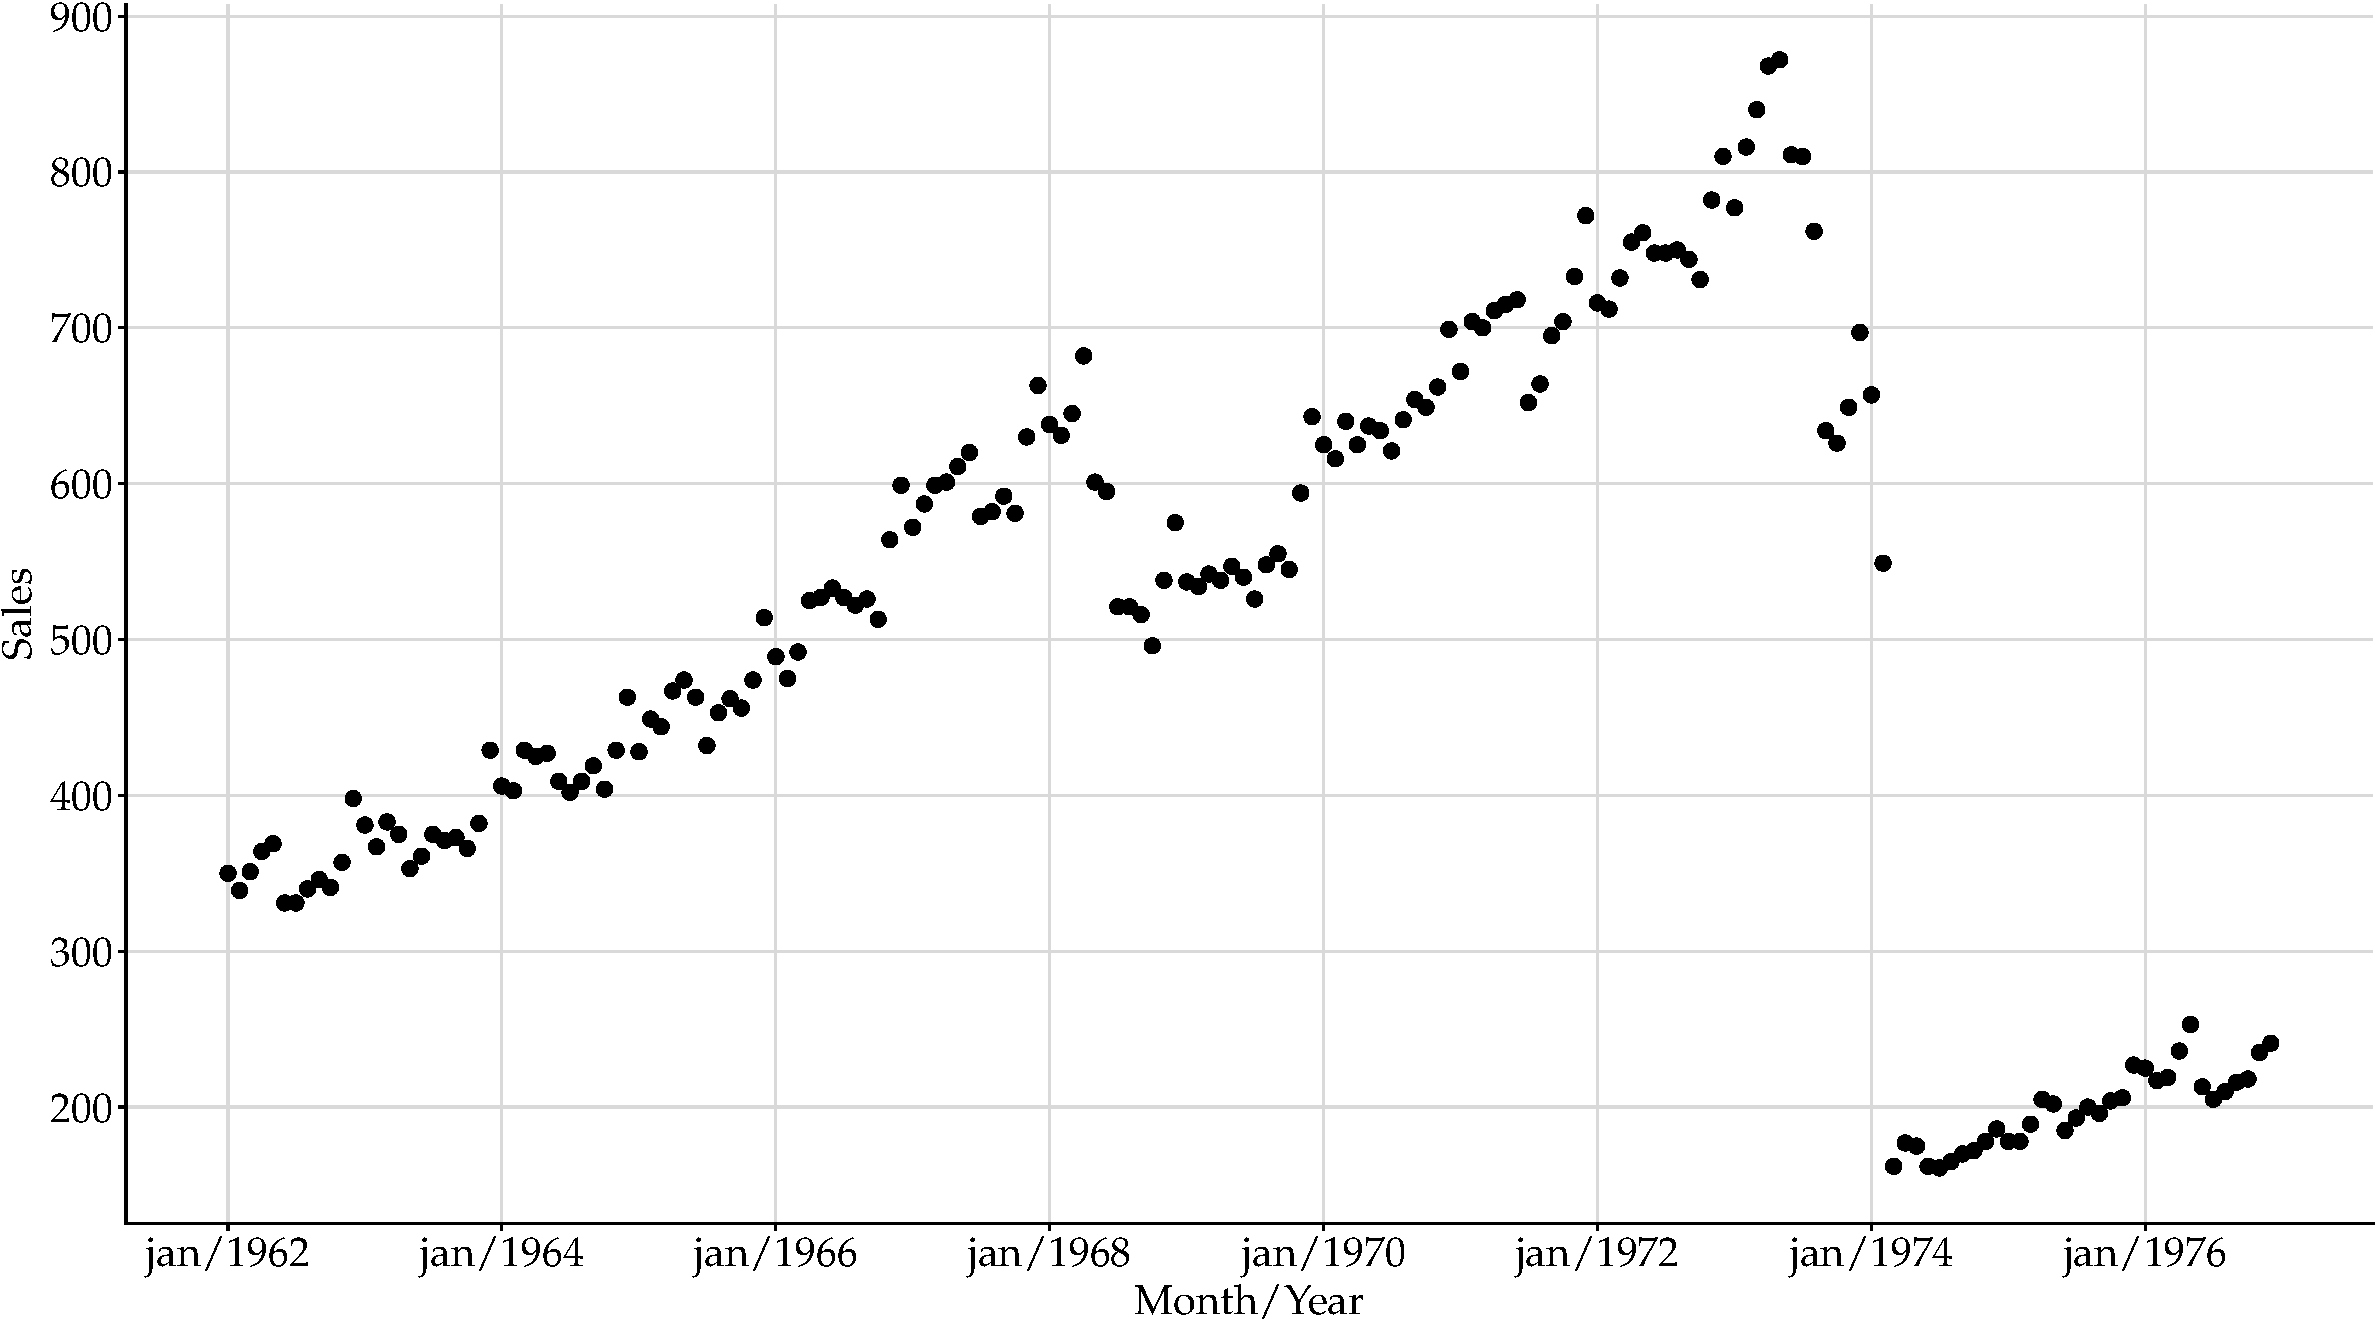
\includegraphics[width=0.9\linewidth]{pybats_detection_files/figure-latex/plot-calls-1} 

}

\caption{Average daily telephone calls to Cincinnati directory assistance}\label{fig:plot-calls}
\end{figure}

The automatic monitoring can be done using the \texttt{Monitoring} class
on objects of class \texttt{pybats.dglm.dlm}.

\begin{Shaded}
\begin{Highlighting}[]
\OperatorTok{\textgreater{}\textgreater{}\textgreater{}}\NormalTok{ a }\OperatorTok{=}\NormalTok{ np.array([}\DecValTok{300}\NormalTok{, }\DecValTok{0}\NormalTok{])}
\OperatorTok{\textgreater{}\textgreater{}\textgreater{}}\NormalTok{ R }\OperatorTok{=}\NormalTok{ np.eye(}\DecValTok{2}\NormalTok{)}
\OperatorTok{\textgreater{}\textgreater{}\textgreater{}}\NormalTok{ np.fill\_diagonal(R, val}\OperatorTok{=}\NormalTok{[}\DecValTok{100}\NormalTok{])}
\OperatorTok{\textgreater{}\textgreater{}\textgreater{}}\NormalTok{ mod }\OperatorTok{=}\NormalTok{ dlm(a, R, ntrend}\OperatorTok{=}\DecValTok{2}\NormalTok{, deltrend}\OperatorTok{=}\FloatTok{0.95}\NormalTok{)}
\OperatorTok{\textgreater{}\textgreater{}\textgreater{}} 
\OperatorTok{\textgreater{}\textgreater{}\textgreater{}} \CommentTok{\# Fit with monitoring}
\OperatorTok{\textgreater{}\textgreater{}\textgreater{}}\NormalTok{ monitor }\OperatorTok{=}\NormalTok{ Monitoring(mod}\OperatorTok{=}\NormalTok{mod, prior\_length }\OperatorTok{=} \DecValTok{20}\NormalTok{, bilateral }\OperatorTok{=} \VariableTok{True}\NormalTok{, }
\OperatorTok{\textgreater{}\textgreater{}\textgreater{}}\NormalTok{ smooth }\OperatorTok{=} \VariableTok{True}\NormalTok{, interval }\OperatorTok{=} \VariableTok{True}\NormalTok{, level }\OperatorTok{=} \FloatTok{0.05}\NormalTok{)}
\end{Highlighting}
\end{Shaded}

where

\begin{itemize}
\tightlist
\item
  \texttt{mod}: A DLM from \texttt{pybats.dglm.dlm};
\item
  \texttt{bilateral}: A Boolean indicating if a bilateral monitoring
  should be performed
\item
  \texttt{prior\_length}: A integer that indicates the number of prior
  observations without monitoring;
\item
  \texttt{smooth}: a Boolean indicating if smooth moments should be
  computed;
\item
  \texttt{interval}: a Boolean indicating if credible intervals should
  be calculated;
\item
  \texttt{level}: A number between 0 and 1 indicating the probability
  level of the credible interval.
\end{itemize}

The \texttt{.fit} method will perform the monitoring steps by the
following arguments

\begin{itemize}
\tightlist
\item
  \texttt{h}: Value of change in the scale or location of the predictive
  distribution.
\item
  \texttt{tau}: The threshold to compare de Bayes factor.
\item
  \texttt{change}: is a list of values to increase the uncertainty on
  state space parameter by multiplying the prior covariance matrix,
  \(\mathbf{R}_t\), when the monitor detects potential outlier or
  parametric change. If length of change var is different to number of
  model parameters, then the covariance matrix is multiplied by the
  first value in the List. The covariance terms are multiplied by the
  minimum value in \texttt{change\ var}.
\end{itemize}

By default we'll use \texttt{tau=0.135} and \texttt{h=4}. For more
details see West and Harrison. A summary for the fit will be
automatically printed, information regarding what was detected (outlier
or parametric change), values for \(H_t\), \(L_t\) and \(l_t\). The
result will be a dictionary with same structure presented in the
smoothing section

\begin{Shaded}
\begin{Highlighting}[]
\OperatorTok{\textgreater{}\textgreater{}\textgreater{}}\NormalTok{ fit\_monitor }\OperatorTok{=}\NormalTok{ monitor.fit(y}\OperatorTok{=}\NormalTok{calls[}\StringTok{"average\_daily\_calls"}\NormalTok{], }
\OperatorTok{\textgreater{}\textgreater{}\textgreater{}}\NormalTok{ h}\OperatorTok{=}\DecValTok{4}\NormalTok{, tau}\OperatorTok{=}\FloatTok{0.135}\NormalTok{, change\_var}\OperatorTok{=}\NormalTok{[}\DecValTok{10}\NormalTok{, }\DecValTok{2}\NormalTok{])}
\end{Highlighting}
\end{Shaded}

\begin{verbatim}
## Upper potential outlier detected at time 24 with H=6.4117e-03, L=6.4117e-03 and l=1
## Upper potential outlier detected at time 36 with H=4.7989e-02, L=4.7989e-02 and l=1
## Upper potential outlier detected at time 48 with H=1.0851e-02, L=1.0851e-02 and l=1
## Upper parametric change detected at time 61 with H=3.7221e+02, L=8.8687e-01 and l=3
## Lower parametric change detected at time 69 with H=7.3680e+01, L=2.1462e+01 and l=3
## Upper parametric change detected at time 73 with H=1.0187e+03, L=5.1939e+00 and l=3
## Lower potential outlier detected at time 77 with H=4.8265e-04, L=4.8265e-04 and l=1
## Lower potential outlier detected at time 79 with H=8.3879e-05, L=8.3879e-05 and l=1
## Upper potential outlier detected at time 84 with H=5.9177e-02, L=5.9177e-02 and l=1
## Upper potential outlier detected at time 95 with H=6.9365e-02, L=6.9365e-02 and l=1
## Upper potential outlier detected at time 108 with H=7.3072e-02, L=7.3072e-02 and l=1
## Lower potential outlier detected at time 115 with H=1.2647e-04, L=1.2647e-04 and l=1
## Lower parametric change detected at time 121 with H=9.8413e+00, L=9.8413e+00 and l=3
## Upper potential outlier detected at time 132 with H=2.8814e-02, L=2.8814e-02 and l=1
## Upper parametric change detected at time 137 with H=1.3818e+00, L=1.5046e-02 and l=3
## Lower potential outlier detected at time 138 with H=9.5186e-03, L=9.5186e-03 and l=1
## Lower potential outlier detected at time 140 with H=2.8420e-02, L=2.8420e-02 and l=1
## Lower potential outlier detected at time 141 with H=1.6058e-03, L=1.6058e-03 and l=1
## Upper potential outlier detected at time 144 with H=1.1479e-01, L=1.1479e-01 and l=1
## Lower potential outlier detected at time 146 with H=1.0036e-05, L=1.0036e-05 and l=1
## Lower potential outlier detected at time 147 with H=1.4096e-08, L=1.4096e-08 and l=1
\end{verbatim}

\begin{Shaded}
\begin{Highlighting}[]
\OperatorTok{\textgreater{}\textgreater{}\textgreater{}}\NormalTok{ forecast\_df }\OperatorTok{=}\NormalTok{ fit\_monitor.get(}\StringTok{"filter"}\NormalTok{).get(}\StringTok{"predictive"}\NormalTok{)}
\end{Highlighting}
\end{Shaded}

\begin{figure}

{\centering 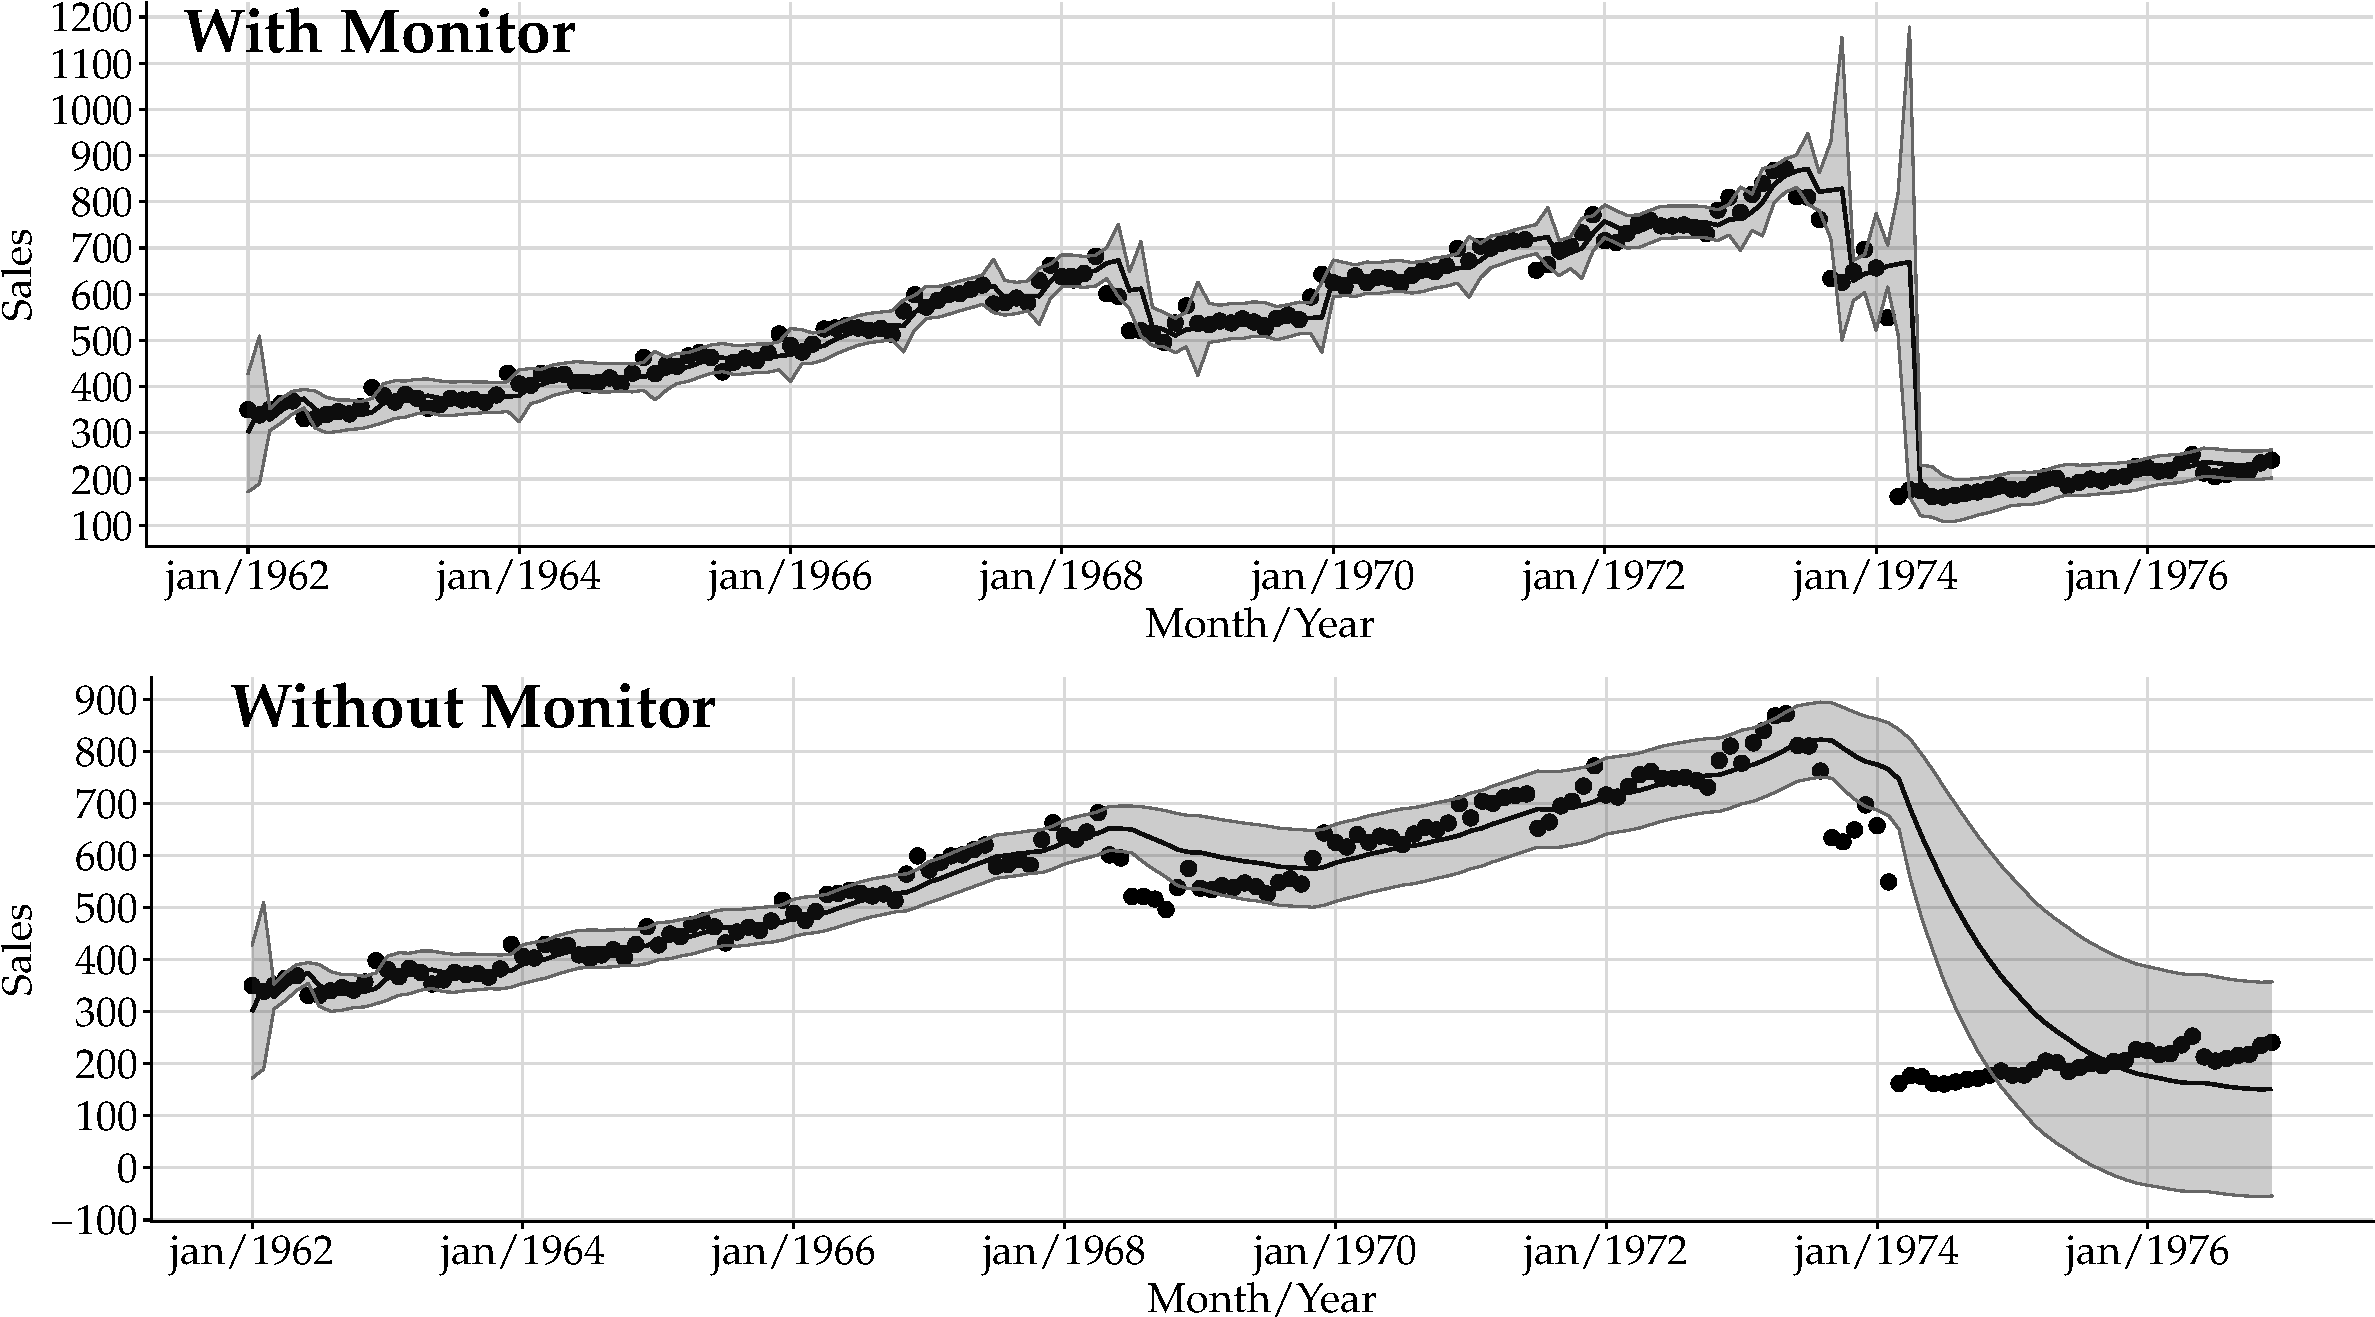
\includegraphics[width=0.9\linewidth]{pybats_detection_files/figure-latex/plot-fit-cp6-filter-monitor-1} 

}

\caption{Mean response for Filtered predictive distribution with $95\%$ credible interval with and without monitor}\label{fig:plot-fit-cp6-filter-monitor}
\end{figure}

\end{document}
